%% 论文 V1（claude 版）
%% 基于《计算机学报》单栏 CjC 模板（Overleaf: latextemplet-CjC-xelatex）
%% 编译方式：XeLaTeX；请将本文件与 figures/、ref.bib 放入模板工程后编译
\documentclass[10.5pt,compsoc,UTF8]{CjC}
\usepackage{CTEX}
\usepackage{graphicx}
\usepackage{footmisc}
\usepackage{subfigure}
\usepackage{url}
\usepackage{multirow}
\usepackage{multicol}
\usepackage[noadjust]{cite}
\usepackage{amsmath,amsthm}
\usepackage{amssymb,amsfonts}
\usepackage{booktabs}
\usepackage{color}
\usepackage{ccaption}
\usepackage{float}
\usepackage{fancyhdr}
\usepackage{caption}
\usepackage{algorithm}
\usepackage{algpseudocode}
\usepackage{xcolor,stfloats}
\usepackage{comment}
\setcounter{page}{1}
\graphicspath{{figures/}}
\usepackage{cuted}
\usepackage{captionhack}
\usepackage{epstopdf}
\usepackage{gbt7714}

%===============================%
\headevenname{\mbox{\quad} \hfill  \mbox{\zihao{-5}{ \hfill 数据推断泄露的集合敏感度审计  } \hspace {50mm} \mbox{2026 年 7 月}}}%
\headoddname{杜浩存 \hfill 摊销层次与闭式读出：可认证的集合敏感度审计}%

\renewcommand{\thefootnote}{\fnsymbol{footnote}}
\setcounter{footnote}{0}
\renewcommand\footnotelayout{\zihao{5-}}

\newtheoremstyle{mystyle}{6pt}{6pt}{\normalfont}{1em}{\bf}{}{1em}{}
\theoremstyle{mystyle}
\newtheorem{definition}{定义}
\newtheorem{observation}{观察}
\newtheorem{proposition}{命题}
\renewcommand\figurename{图~}
\renewcommand{\thesubfigure}{(\alph{subfigure})}
\newcommand{\upcite}[1]{\textsuperscript{\cite{#1}}}
\renewcommand{\labelenumi}{(\arabic{enumi})}
\newcommand{\tabincell}[2]{\begin{tabular}{@{}#1@{}}#2\end{tabular}}
\renewcommand{\bibsection}{}
\makeatletter
\renewcommand{\@biblabel}[1]{[#1]\hfill}
\makeatother
\setlength\parindent{2em}

\newcommand{\syn}{\mathrm{syn}}
\newcommand{\Rtwo}{R^{2}}

\begin{document}

\hyphenpenalty=50000
\thispagestyle{plain}%
\thispagestyle{empty}%
\pagestyle{CjCheadings}

\vspace {-13mm}
\onecolumn
\zihao{5-}\noindent 杜浩存 \hfill 研究论文\hfill 2026 年 7 月\\
\noindent\rule[0.25\baselineskip]{\textwidth}{1pt}

{
\centering
\vspace {11mm}
{\zihao{2} \heiti 摊销层次与闭式读出：\\面向数据推断泄露的可认证集合敏感度审计}

\vskip 5mm

{\zihao{4}\fangsong 杜浩存}

\vspace {5mm}

\zihao{5}{(西安交通大学\quad 西安\quad 710049)}
}

\vspace {8mm}

\zihao{5}{
\setlength{\baselineskip}{18pt}\selectfont{
\noindent {\heiti 摘\quad 要\quad }
数据推断泄露的风险是可见字段\textbf{集合}上的集合函数 $v_c(S)$——攻击者拿到子集 $S$ 后针对 $S$ 重训所能达到的推断精度上限。子集空间达 $2^{44}$，逐集合重训不可行，因而必须\textbf{摊销}：用一个共享模型回答所有子集查询。本文首先给出一个负面诊断：这种“全摊销”的误差并非随机分布，而是\textbf{系统性地集中在最危险的强协同集合上}。在 PJM 数据的 11352 条重训真值上，共享读出 oracle 的全局排序相关为 0.606，但真值最强的 100 个协同上排序相关坍缩至 0.130，最强档平均低估 0.124；三个排除性对照（逐集合仿射校准只把尾部相关修到 0.199、集成方差在最强档失明、三个独立种子结论一致）表明这是\textbf{表达力与共享参数干涉造成的系统性偏差}，而非尺度漂移或训练噪声。本文将其归因于摊销层次错配：$v_c(S)$ 是内层优化的\textbf{最优值}，而摊销间隙恰在“最优解离共享平均解最远”的实例上最大，强协同正属此类。据此提出把摊销层次由“值”上移到“表示”：主干 $\varphi_\theta(x\odot m_S,\,m_S)$ 摊销条件特征，读出权重按集合闭式重解 $\beta_{S,c}=(\Phi^{\top}\Phi+\lambda I)^{-1}\Phi^{\top}Y_c$。直接复用现成主干（零训练）即把尾部排序相关由 0.130 提升至 0.781、最强档低估由 0.124 降至 0.016，性能超过 50 步查询微调而快 22.4 倍；把闭式头放进训练回路进一步提升至 0.858。在此基础上给出“摊销扫描—配对 FDR—重训认证”三层管线，并坚持“重训真值只用于评估与认证、绝不进入查询路径”的方法学红线。高阶实验给出一个被认证推翻的反例：手工多项式字典在五阶报出 441 个强协同，重训认证后\textbf{无一为真}、与随机对照无统计差异；而学出的表示在同一空间全枚举 108.6 万个集合，自选 top 经认证 10 个为真。由此定标出真值版衰减律（三至五阶最强协同 $0.455\to0.196\to0.154$，密度每阶降约一个数量级），并证明跨独立种子的\textbf{秩一致性}可把候选精确率由 45\% 提升至 100\%——对付共享摊销偏差须用秩统计而非集成方差。全部结论在第二个电网数据集（CAISO）上完整复现：方法阶梯同构（尾部 $0.596\to0.931\to0.969$）、自选候选认证精确率 95\%、字典在五阶系统性膨胀 1.7 倍且无一为真、衰减律更陡（$0.294\to0.157\to0.104$）。最后用注入已知强度的纯高阶信号定标出管线的可认证边界 $k^\ast=5$。本文把 $k\ge6$ 的成因逐层剥开：合成信号上六、七阶卡在表示的分布外、八阶起是样本量硬墙；据此改造元训练分布可把六阶注入命中率由 $32\%$ 提到 $75\%$，\textbf{但该增益在真实机密字段上完全不迁移}（认证均值 $0.031\to0.016$）。配对认证协议进一步排除了"噪声底源于选择偏差"与"饱和压缩"两种解释。真正的原因是：\textbf{随机抽取的六、七阶集合本身即带显著大于零的协同增量}（$0.031$ 与 $0.022$，$p<10^{-4}$），高阶协同弱而普遍、\textbf{没有强尾可供搜索}——六阶上诸多改进无效，不是因为"找不到"，而是因为"没有值得找的"。由此得到两条措辞纪律："最危险的协同是低阶的"须限定为"在可认证范围内"（外推七阶最强协同仍在显著阈之上，应表述为"存在但不可认证"）；注入定标给出的是能力上界而非真实性能预期。同一定标也表明认证这把尺子本身随阶衰减，故所报衰减律的倍数应读作下界。
\par}}
\vspace {5mm}

\zihao{5}{\noindent
{\heiti 关键词 \quad }数据推断泄露；集合函数；摊销优化；闭式读出；协同效应；假发现率；可认证审计
}

\vskip 7mm

\begin{center}
\zihao{3}{ \heiti Amortization Level and Closed-Form Readout: Certifiable Set-Sensitivity Auditing for Data Inference Leakage}\\
\vspace {5mm}
\zihao{5}{ DU Hao-Cun}\\
\vspace {2mm}
\zihao{5-}{{(Xi'an Jiaotong University, Xi'an 710049, China)}}
\end{center}

\zihao{5}{
\setlength{\baselineskip}{18pt}\selectfont{
{\bf Abstract}\quad
The risk of data inference leakage is a set function $v_c(S)$ over subsets of visible fields: the best inference accuracy an attacker can reach by retraining on $S$. With $2^{44}$ subsets, per-subset retraining is intractable, so the mapping must be \emph{amortized} into a single shared model. This paper first reports a negative diagnosis: the error of such full amortization is not random but \emph{systematically concentrated on the most dangerous, strongly synergistic subsets}. On 11352 retraining ground-truth entries from PJM data, a shared-readout oracle attains a global rank correlation of 0.606, yet on the 100 strongest true synergies the rank correlation collapses to 0.130 with an average underestimation of 0.124. Three control experiments---per-subset affine recalibration lifts the tail correlation only to 0.199, ensemble variance is flat on the strongest band, and three independent seeds agree---show this is a \emph{systematic bias from limited expressiveness and shared-parameter interference}, not a scale drift or training noise. We attribute it to a mismatch in the amortization level: $v_c(S)$ is the \emph{optimal value} of an inner optimization, and the amortization gap is largest precisely where the per-instance optimum is farthest from the shared average solution---which is what strong synergy is. We therefore lift amortization from the value to the representation: a backbone $\varphi_\theta(x\odot m_S, m_S)$ amortizes conditional features while readout weights are re-solved per subset in closed form, $\beta_{S,c}=(\Phi^{\top}\Phi+\lambda I)^{-1}\Phi^{\top}Y_c$. Reusing an off-the-shelf backbone with zero training raises the tail rank correlation from 0.130 to 0.781 and cuts the strongest-band underestimation from 0.124 to 0.016, outperforming 50-step query-time fine-tuning while being 22.4$\times$ faster; training with the closed-form head in the loop further raises it to 0.858. We then give a three-tier pipeline---amortized scan, paired FDR test, retraining certification---under the methodological red line that retraining truth is used only for evaluation and certification, never inside the query path. A certified counterexample follows: a handcrafted polynomial dictionary reports 441 strong fifth-order synergies of which \emph{none} survives retraining certification (indistinguishable from a random control), whereas the learned representation, enumerating all 1.086 million fifth-order subsets, yields a self-selected top list with 10 certified true synergies. This calibrates a certified decay law (strongest synergy $0.455\to0.196\to0.154$ from third to fifth order, density dropping about one order of magnitude per level) and shows that \emph{rank agreement across independently retrained seeds} raises candidate precision from 45\% to 100\%---shared amortization bias must be attacked with rank statistics rather than ensemble variance. All conclusions replicate on a second grid dataset (CAISO): an isomorphic method ladder ($0.596\to0.931\to0.969$ on the tail), 95\% certified precision of self-selected candidates, systematic 1.7$\times$ inflation of the dictionary at fifth order with zero true positives, and a steeper decay law ($0.294\to0.157\to0.104$). Finally, injecting pure higher-order signals of known strength calibrates the pipeline's certifiable ceiling at $k^\ast=5$ and separates the failure beyond it into two regimes: at orders six and seven the bottleneck is representational---a target-agnostic dictionary containing the generating monomial still ranks the same signals first among 400 random same-order sets---whereas from order eight on it is a statistical wall set by sample size. The same calibration shows that the certification ruler itself attenuates with order, so the reported decay factors should be read as lower bounds.
\par}}
\vspace {5mm}

{{\bf Keywords}\quad data inference leakage; set function; amortized optimization; closed-form readout; synergy; false discovery rate; certifiable auditing\par}

\zihao{5}
\vskip 10mm

%%%%%%%%%%%%%%%%%%%%%%%%%%%%%%%%%%%%%%%%%%
\section{\heiti 引言}

电网、金融、医疗等领域的运行数据在跨主体共享前通常只做“删除机密字段”这一步脱敏，但保留字段之间由物理定律与统计规律决定的耦合，使攻击者仍能用公开字段训练推断模型间接恢复被删除的量，即数据推断泄露（Data Inference Leakage, DIL）\upcite{hu2026ignn}。已有工作多为\textbf{每个字段}输出一个标量敏感度分数，而泄露的本质是字段\textbf{集合}的属性：存在大量“单看安全、合体泄露”的组合。以本文 PJM 数据为例，风电出力与风电占比各自单独推断总发电量的测试 $\Rtwo$ 仅 0.064 与 0.162，两者同时可见时跃升至 0.928——因为总量在物理上等于出力除以占比。因此敏感度评估必须升维为定义在任意字段集合上的集合函数 $v_c(S)$。

升维之后的困难在于\textbf{评估成本}。忠实的 $v_c(S)$ 要求“攻击者最优响应”语义，即对每个 $S$ 从头重训攻击者至最优；44 个字段的子集空间达 $2^{44}\approx1.8\times10^{13}$，而单次重训需分钟级开销。唯一现实的出路是\textbf{摊销}：训练一个以可见性掩码为条件的共享模型，一次前向回答任意子集查询。这正是摊销优化\upcite{amos2023amortized}与摊销归因\upcite{jethani2022fastshap,covert2023vitshapley}的标准范式，在本文的前置工作中也确实把单集合评估成本从分钟级降到毫秒级。

然而本文的出发点是一个负面观察：\textbf{这种摊销在最需要它准的地方最不准}。图 \ref{fig:tail} 左给出直观证据——共享读出 oracle 在全体 11352 条重训真值上排序相关 0.606 看似可用，但把视野限制到真值最强的 100 个协同（安全审计唯一真正关心的那一档），排序相关坍缩到 0.130，估计值几乎与真值无关。换言之，一个“平均意义上不错”的摊销估计器，在尾部是失明的。若不修正，基于它的一切风险排序、防护集选择与高阶搜索都建立在流沙之上。

本文认为这不是工程调参问题，而是\textbf{摊销层次}的错配。$v_c(S)$ 是一个内层优化问题的\textbf{最优值}（value function），而摊销间隙的已知性质是：在“逐实例最优解离共享平均解最远”的实例上最大\upcite{cremer2018inference,amos2023amortized}；强协同集合恰恰是这种实例——它要求模型实现一个仅在该子集上成立的精确配合（如除法电路），而这种掩码在训练中出现概率极低。更关键的是，协同 $\syn=v(S)-\max_T v(T)$ 是两个同量级数的差，误差为两个间隙之差，而间隙在强协同 $S$ 上大、在其平庸父集 $T$ 上小，于是协同被\textbf{系统性压低}。

据此，本文把摊销层次从“值”上移到“表示”：让共享主干只负责摊销\textbf{条件特征} $\varphi_\theta(x\odot m_S,m_S)$，而把读出权重按集合闭式重解。这一改动使每个子集拥有自己的、不与其他子集共享的解，从而消除干涉；同时保留一次前向的摊销效率，因为闭式解只是一个小规模线性系统。实验表明，即便完全复用为共享读出训练的现成主干（零额外训练），尾部排序相关就从 0.130 升到 0.781、最强档低估从 0.124 降到 0.016，且超过 50 步查询微调的效果而快 22.4 倍。

有了可靠的估计器，才谈得上在指数空间里做发现。本文给出“摊销扫描—配对 FDR—重训认证”三层管线，并在全程坚持一条方法学红线：\textbf{重训真值只用于评估与认证，绝不进入查询、路由或校准路径}——否则“估计器有多准”会退化为不可证伪的循环论证。该管线在高阶实验中给出了一个有警示意义的结果：手工多项式字典在五阶报出 441 个 $\syn>0.2$ 的“强协同”，重训认证后\textbf{无一为真}，与随机对照组无统计差异（$p=0.058$）；而学出的表示全枚举同一空间的 108.6 万个集合后零个 $\syn>0.2$，其自选 top-21 经认证有 10 个为真。这说明高阶发现的瓶颈不在搜索策略而在\textbf{估计器的可信度}。

本文主要贡献如下：

(1) \textbf{诊断}。指出并量化全摊销集合敏感度估计的\textbf{尾部失明}现象，用三个排除性对照证明其为系统性偏差而非噪声或尺度问题，并以“值函数摊销间隙”给出机制归因（第 4 节）。

(2) \textbf{方法}。提出摊销表示 + 逐集合闭式读出，给出零训练（L0）与元训练（L1）两个实例，并把手工字典、L0、L1、微调统一为沿“表示适应程度”排列的连续谱；配合三层审计管线与方法学红线（第 5 节）。

(3) \textbf{实验与定标}。在两个真实电网数据集上系统验证：尾部保真度、成本、高阶认证对决、真值版衰减律、跨种子秩一致性过滤；并给出对既有手工字典方法的\textbf{认证级证伪}（第 6 节）。

%%%%%%%%%%%%%%%%%%%%%%%%%%%%%%%%%%%%%%%%%%
\section{\heiti 相关工作}

\textbf{数据敏感度评估}。IGNN\upcite{hu2026ignn} 将电网字段间推断关系组织为图，用图注意力网络输出字段级敏感度，是本文的直接背景。本文与其的根本差别在于输出粒度（单字段分数升维为任意集合的集合函数）与测量口径（固定模型下的风险传播改为逐集合重训的最优响应）。

\textbf{特征子集贡献与高阶交互}。SHAP\upcite{lundberg2017shap} 与交互指标的公理化\upcite{grabisch1999interaction} 刻画\textbf{固定模型}在特征扰动下的行为；FastSHAP\upcite{jethani2022fastshap}、ViT-Shapley\upcite{covert2023vitshapley} 用摊销网络加速归因。这些方法摊销的是\textbf{标量归因值}，正是本文诊断为尾部失明的“值摊销”。ProxySPEX\upcite{kang2024proxyspex} 等高阶交互搜索依赖层级性假设（高阶交互的低阶子集也显著）以控制搜索代价；本文的可靠估计器使五阶以内可直接全枚举，从而把层级假设的适用性问题转为可测量的漏检率。Datamodels\upcite{ilyas2022datamodels} 在训练数据维度拟合“子集 $\mapsto$ 性能”，与本文在特征维度的工作平行。

\textbf{摊销优化与闭式基学习器}。摊销间隙及其在“难实例”上放大的性质在变分推断\upcite{cremer2018inference}与摊销优化综述\upcite{amos2023amortized}中已有讨论，本文把它迁移到集合函数估计并给出安全语义下的后果。R2D2\upcite{bertinetto2019r2d2} 与 MetaOptNet\upcite{lee2019metaoptnet} 在小样本\textbf{分类平均准确率}上使用可微闭式基学习器；本文把同一机制用于\textbf{集合函数的尾部}——在安全审计里恰好只有尾部重要——并给出“摊销间隙集中在哪类实例”的定位与认证证据。LQF\upcite{achille2021lqf} 与神经正切核\upcite{jacot2018ntk} 提供“凸化适应”的相关背景，但它们改造损失与整个模型，本文只重解读出层，零训练即用。

\textbf{任意条件建模}。VAEAC\upcite{ivanov2019vaeac}、ACFlow\upcite{li2020acflow}、GRAPE\upcite{you2020grape} 学习任意观测子集条件化的模型，本文在“随机掩码训练”机制上与之同源，但目标是集合函数的忠实估计而非数据分布建模。多重检验方面，本文采用 Benjamini--Hochberg 程序\upcite{benjamini1995fdr} 控制假发现率。

%%%%%%%%%%%%%%%%%%%%%%%%%%%%%%%%%%%%%%%%%%
\section{\heiti 问题形式化}

\subsection{威胁模型}

设数据表含字段集 $F$，其中规程认定的机密字段集为 $C\subset F$，其余为一般字段集 $G=F\setminus C$（本文两个数据集均为 $|G|=44$、$|C|=12$）。共享时机密字段被删除，攻击者获得某可见集合 $S\subseteq G$ 的完整列数据，并假设其拥有同分布历史样本、知晓字段语义、可从任意模型族训练推断模型。这是对攻击者有利的保守假设，据此得到的是风险上界。防御方目标：对任意拟共享集合 $S$，评估每个机密字段被推断的风险，并定位构成协同泄露的字段组合。

\subsection{集合敏感度与不可约协同}

\begin{definition}[集合敏感度]
给定机密字段 $c\in C$ 与可见集合 $S\subseteq G$，
\begin{equation}
v_c(S)=\max\Bigl(0,\ \sup_{g\in\mathcal{G}} \Rtwo_{\mathrm{test}}\bigl(g(X_S);\,x_c\bigr)\Bigr),
\label{eq:vcs}
\end{equation}
其中 $X_S$ 为仅保留 $S$ 中字段的数据，上确界取在模型族与训练过程之上。
\end{definition}

式 (\ref{eq:vcs}) 的上确界语义是\textbf{攻击者最优响应}：对每个 $S$ 攻击者从头重训至最优。这一点是本文全部方法论的支点——它意味着 $v_c(S)$ 是一个\textbf{内层优化问题的最优值}，而不是某个固定模型的读数。第 4 节将说明，正是这一“最优值”属性决定了全摊销失效的形态。

\begin{definition}[$k$ 阶不可约协同]
对 $|T|=k\ge2$，
\begin{equation}
\syn_k^c(T)=v_c(T)-\max_{T'\subset T,\,|T'|=k-1} v_c(T'),\qquad
\syn_k(T)=\max_{c\in C}\syn_k^c(T).
\label{eq:synk}
\end{equation}
\end{definition}

采用“减去最优低阶子集”而非全交互展开源于安全语义：防御者关心“同时放行 $T$ 是否比放行其任何真子集更危险”。注意 $\syn$ 是两个同量级数的\textbf{差分}，这一结构在第 4 节被证明是尾部失明的放大器。

\subsection{测量口径、噪声底与方法学红线}

本文以\textbf{重训}为唯一真值口径：对每个待测集合从头训练专用推断模型并实测保留集 $\Rtwo$。同集合不同种子重复重训的复现噪声底实测 $\sigma\approx0.002$--$0.004$，据此取协同显著阈 $\syn>0.10$（约噪声底 25 倍以上）。

数据被切分为训练集、\textbf{搜索片}（search）与\textbf{审计片}（audit）三部分：所有自适应选择（选哪个机密字段、选哪个最强父集、选哪些候选）只允许在搜索片上做，审计片只用于最终报数与检验，以避免选择性推断带来的赢家诅咒。

最后，本文坚持一条\textbf{方法学红线}：重训真值只允许出现在评估与认证环节，\textbf{绝不允许进入查询、路由或校准路径}。理由是部署时数据持有方并没有任何真值可用；一旦把真值塞进查询路径，“估计器逼近得多准”就变成不可证伪的循环论证。本文在方案设计阶段以“承认性检查”执行该红线：把估计器拿掉、只留真值查表，看效果还剩多少——若大部分效果来自查表本身，该方案即被否决。

%%%%%%%%%%%%%%%%%%%%%%%%%%%%%%%%%%%%%%%%%%
\section{\heiti 诊断：全摊销为何在最危险处失效}

\subsection{现象：尾部失明}

全摊销 oracle 的标准形态是：主干接收 $[x\odot m_S,\,m_S]$，经共享读出层输出对 $|C|$ 个机密字段的预测，训练时用随机子集失活遍历掩码空间。这一设计在平均意义上是成功的：在 PJM 的 11352 条 $(i,j,c)$ 重训真值上，其协同估计与真值的 Spearman 相关为 0.606。

但把视野收缩到尾部，结论完全反转。图 \ref{fig:tail}(左) 中红色点为真值最强的 100 个协同：它们的估计值大量塌陷到 0 附近，与真值几乎无关，尾部 Spearman 仅 \textbf{0.130}；真值 top-10 的集合在估计排序中的中位名次是 \textbf{6527}（共 11352 条）。分档统计（图 \ref{fig:ladder}(a)）给出更清晰的形态：弱档（真值 $<0.1$）平均低估 0.007，中档 0.037，而强档（真值 $>0.2$）平均低估 \textbf{0.124}——低估量随真值强度单调放大。这正是安全审计最不能接受的失效模式：越危险的组合，越被判为安全。

\subsection{三个排除性对照}

尾部失明可能有三种平凡解释，本文逐一排除。

\textbf{(1) 是不是尺度漂移？} 若 oracle 只是输出的尺度或偏置有系统性漂移，那么逐 $(S,c)$ 的两参数仿射校准 $a\cdot\hat{v}+b$（$a,b$ 在训练集上最小二乘拟合）应当能补回大部分。实测仿射校准把全局相关从 0.606 提到 0.676，但尾部相关只从 0.130 提到 \textbf{0.199}，真值 top-10 的中位名次反而从 6527 退到 8871。结论：这是\textbf{表达力}问题，不是尺度问题。

\textbf{(2) 是不是训练噪声？} 若失效源于随机性，同族集成的方差 $\sigma$ 应在失效处变大，从而可用“不确定度路由”识别。但实测集成方差在最强档是\textbf{平的}——因为所有集成成员共享同一结构性偏差，方差看不见它。结论：这是\textbf{系统性偏差}，标准的不确定度路由在此原理性失效。

\textbf{(3) 是不是某次训练的偶然？} 三个独立种子训练的 oracle 给出一致的尾部失明形态（第 6.8 节的第二数据集也复现同一形态）。结论：这是该架构的稳定属性。

\subsection{机制：值函数的摊销间隙}

排除平凡解释后，本文给出机制归因。$v_c(S)$ 由式 (\ref{eq:vcs}) 定义为内层优化的最优值，全摊销相当于用一组共享参数 $\theta$ 去逼近全部 $2^{|G|}$ 个子集各自的最优解 $g_S^{*}$。摊销优化文献指出，摊销间隙 $\Delta(S)=v_c(S)-\hat{v}_{\theta}(S)$ 在\textbf{最优解离共享平均解最远}的实例上最大\upcite{cremer2018inference,amos2023amortized}。强协同集合正是这类实例：它要求模型实现一个仅在该特定子集上成立的精确配合（例如“出力除以占比得总量”），而该掩码在随机子集失活训练中出现的概率仅万分之几。

更致命的是协同的\textbf{差分结构}。由式 (\ref{eq:synk})，
\begin{equation}
\widehat{\syn}_k(T)-\syn_k(T)=\Delta(T')-\Delta(T),
\label{eq:gapdiff}
\end{equation}
其中 $T'$ 为最强低阶子集。强协同 $T$ 上 $\Delta(T)$ 大、平庸父集 $T'$ 上 $\Delta(T')$ 小，故差值为负且随协同强度放大——协同被系统性压低。两个 0.8 量级的数相减得到 0.1 量级的量，任何在被减数上的系统性偏差都会被放大到结果中。

\begin{figure*}[htbp]
\centering
\centerline{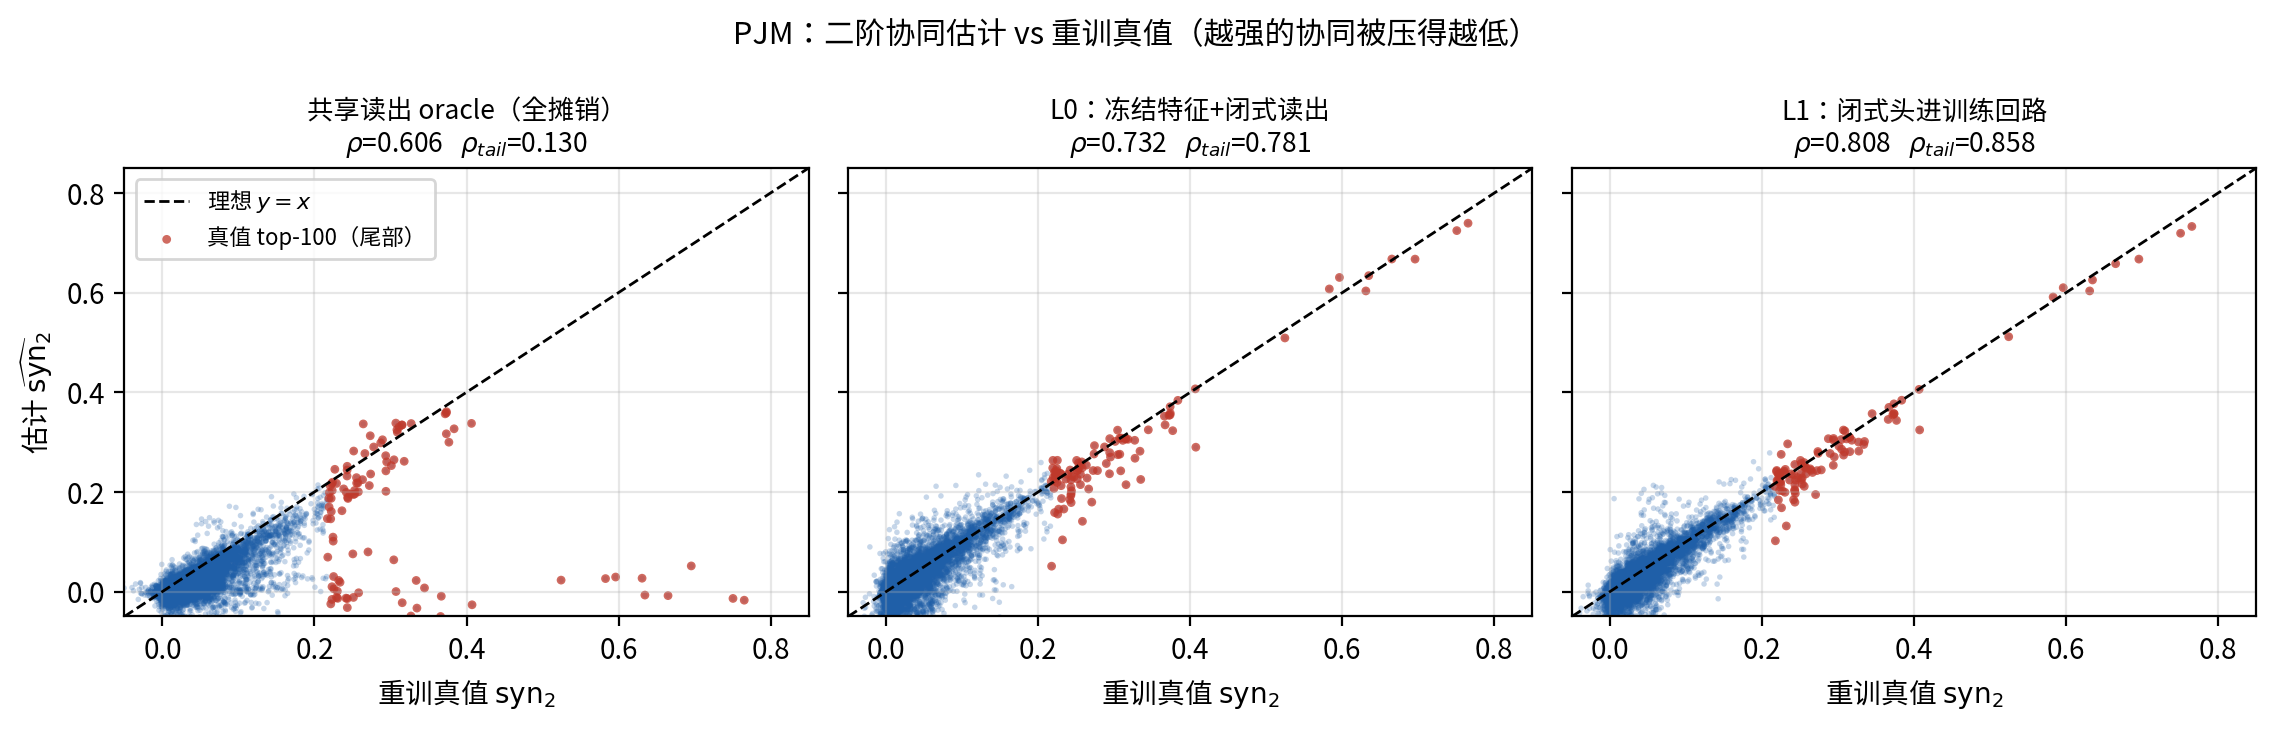
\includegraphics[width=0.99\linewidth]{tail_blindness.png}}
{\heiti 图 1\quad PJM 二阶协同：估计 vs 重训真值（11352 条）。红点为真值 top-100。左：共享读出 oracle 的尾部塌陷（$\rho_{tail}=0.130$）；中：冻结主干 + 闭式读出（零训练，$0.781$）；右：闭式头进训练回路（$0.858$）}
\label{fig:tail}
\end{figure*}

%%%%%%%%%%%%%%%%%%%%%%%%%%%%%%%%%%%%%%%%%%
\section{\heiti 方法：摊销表示与闭式读出}

\subsection{核心思想}

诊断指向的修复方向是明确的：既然失效源于\textbf{读出权重被所有子集共享}，那就让读出权重按集合独有。但若为每个子集单独训练读出层，就退回了逐集合优化的高成本。本文的做法是让读出层\textbf{有闭式解}——岭回归。于是（图 \ref{fig:framework}）：
\begin{align}
\Phi_S &= \varphi_\theta\bigl(X\odot m_S,\ m_S\bigr) \in\mathbb{R}^{n\times d}, \label{eq:phi}\\
\beta_{S,c} &= \bigl(\Phi_S^{\top}\Phi_S+\lambda I\bigr)^{-1}\Phi_S^{\top}\,y_c, \label{eq:ridge}\\
\hat{v}_c(S) &= \max\Bigl(0,\ 1-\tfrac{\|y_c^{\mathrm{ev}}-\Phi_S^{\mathrm{ev}}\beta_{S,c}\|^2}{\|y_c^{\mathrm{ev}}-\bar{y}_c\|^2}\Bigr). \label{eq:r2}
\end{align}
主干 $\varphi_\theta$ 仍然摊销（一次前向对所有子集共享），但式 (\ref{eq:ridge}) 的 $\beta_{S,c}$ 是\textbf{每个 $(S,c)$ 独有的}，不与任何其他子集共享参数，因而不受干涉。计算上，每次查询只需一次前向加一个 $d\times d$ 线性系统求解，仍是毫秒量级。

正则系数 $\lambda$ 在训练集内部再切分的拟合/验证片上逐 $(S,c)$ 独立选取（网格 $10^{-3}$ 至 $10^{2}$），随后用全部训练数据重拟合、在审计片上评估——评估片从不参与 $\lambda$ 选择或拟合。

\subsection{两个实例：L0 与 L1}

\textbf{L0（零训练）}：直接取现成 oracle 主干的倒数第二层激活作为 $\varphi$，主干完全冻结。这是最保守的实例——它不需要任何额外训练，唯一的改动就是把最后一层从“共享权重”换成“逐集合闭式解”，因而构成一个单变量受控对照，可以干净地把收益归因于读出层而非别的因素。

\textbf{L1（元训练）}：把闭式头放进训练回路，梯度反传穿过式 (\ref{eq:ridge}) 的求解算子，$\lambda$ 以对数参数化与主干联合学习（R2D2/MetaOptNet 式\upcite{bertinetto2019r2d2,lee2019metaoptnet}）。动机是：L0 的主干是为共享读出训练的，它并不知道自己的读出层将被逐集合重解，于是仍把容量花在“记住每个掩码该输出什么”而非“造一组好重解的基”。每个元步骤采样若干掩码，每个掩码从训练集抽 support 与 query 两批样本，用 support 闭式求解、在 query 上算损失。

\subsection{统一视角}

本文指出，四类方法是\textbf{同一框架沿“表示适应程度”排列的四个点}：手工多项式字典（$\varphi$ 冻成固定基）、L0（$\varphi$ 为冻结的学习表示）、L1（$\varphi$ 为面向重解而元训练的表示）、查询时微调（$\varphi$ 与 $\beta$ 都动）。这一视角的价值在于：手工字典不是“另一类方法”，而是本框架的\textbf{退化情形}；第 6.4 节将证明这个退化情形在高阶上会系统性地报假。

\begin{figure*}[htbp]
\centering
\centerline{
\includegraphics[width=0.99\linewidth]{framework.png}}
{\heiti 图 2\quad 方法总览。上：摊销层次由“值”上移到“表示”，读出权重逐集合闭式重解；下：三层审计管线与方法学红线}
\label{fig:framework}
\end{figure*}

\subsection{三层审计管线}

估计器可靠之后，发现流程组织为三层（图 \ref{fig:framework} 下半）：

\textbf{第 1 层：摊销扫描}。用 L1 对目标阶数做\textbf{全枚举}（本文 $k\le5$，五阶空间 $\binom{44}{5}=1086008$），单集合约 2.5 ms，四卡约 13 分钟扫完。输出按 $\syn$ 降序的候选榜。注意全枚举使得“层级搜索是否漏检”这一长期困扰高阶交互发现的问题在 $k\le5$ 被\textbf{消解而非绕过}。

\textbf{第 2 层：配对检验与 FDR}。闭式读出的一个结构性优势是：$S$ 与其父集 $T$ 的预测误差来自\textbf{同一个 $\varphi$、同一批审计样本}，可逐样本配对，且闭式解没有优化噪声（微调则两边各带独立的初始化与批序噪声，差分方差放大 $\sqrt{2}$）。构造逐样本配对差 $d_i=e_T^2(i)-e_S^2(i)$，检验 $H_0:\syn\le\tau$，单边 $t$ 检验后做 BH-FDR\upcite{benjamini1995fdr}。选择（选 $c$、选最强父集）在搜索片完成，$p$ 值只在审计片算一次。

\textbf{第 3 层：重训认证}。对 top-$K$ 候选（及随机对照组）逐个重训专用模型：对 $|S|=m$ 的集合重训 $1+m$ 个模型（$S$ 自身与全部 $m-1$ 阶子集），得 $\syn$ 的重训真值。早停使用\textbf{训练集内部}划出的验证片，测试集完全不参与训练与早停。这一层昂贵（约 160 s/集合）但忠实，是唯一被允许写进结论的口径。

\begin{algorithm}[htbp]
\caption{三层协同发现与认证}
\label{alg:pipeline}
\begin{algorithmic}[1]
\Require 数据 $X$、机密集 $C$、阶数 $k$、阈值 $\tau$、认证预算 $K$
\State 训练 L1 主干 $\varphi_\theta$（随机子集失活 + 闭式头在回路内）
\ForAll{$|S|=k$ 与其全部 $(k{-}1)$ 阶子集}
  \State 由式 (\ref{eq:phi})--(\ref{eq:r2}) 算 $\hat{v}_c(S)$，得 $\widehat{\syn}_k(S)$ \Comment{全枚举，$\sim2.5$ ms/集合}
\EndFor
\ForAll{候选 $S$}
  \State 在\textbf{搜索片}选 $c^\star$ 与最强父集 $T^\star$
  \State 在\textbf{审计片}算配对 $t$ 统计量与 $p$ 值（$H_0:\syn\le\tau$）
\EndFor
\State BH-FDR（$q=0.05$）得统计保证清单 $\mathcal{L}$
\State 从 $\mathcal{L}$ 取 top-$K$ 与随机对照组，逐个\textbf{重训认证}
\State \Return 认证清单与 Mann--Whitney 组间检验结果
\end{algorithmic}
\end{algorithm}

%%%%%%%%%%%%%%%%%%%%%%%%%%%%%%%%%%%%%%%%%%
\section{\heiti 实验}

\subsection{实验设置}

\textbf{数据集}。主数据集为 PJM 区域 2025 年小时级运行数据（8760 行，清洗后 6556 行有效），44 个一般字段、12 个机密字段（含总发电量、计量负荷、净/毛交换功率、系统损耗、日前与实时阻塞价格、边际损耗价格、日前总电价、三类备用总量）。第二数据集为 CAISO 2025 年小时级数据（8760 行，清洗后 8722 行），原始 307 列经字段设计收缩为同样的 44+12 结构（详见 6.8 节）。两者均按 7:3 随机切分训练与保留集，保留集再对半切分为搜索片与审计片。

\textbf{真值}。二阶真值为全部 44 个单字段与 946 个字段对逐个重训（990 次），三阶为随机抽取的无偏三元组池，四、五阶为候选与对照的逐集合认证。重训协议：专用多层感知机（两隐层 128 维、dropout 0.15）、Adam（$10^{-3}$，权重衰减 $5\times10^{-4}$）、最多 400 轮、耐心 120 轮，早停用训练集内部 15\% 验证片。

\textbf{指标}。全局排序相关 $\rho$（Spearman）、\textbf{尾部排序相关} $\rho_{tail}$（真值 top-100 内部）、分档低估量 gap（真值减估计）、真值 top-10 的估计排名中位数、认证精确率（top-$K$ 中真值 $>0.10$ 的比例）。

\subsection{RQ1：尾部失明及其修复}

表 \ref{tab:ladder} 给出全空间（11352 条）上沿“表示适应程度”排列的方法阶梯。共享读出 oracle 的全局相关尚可（0.606）而尾部坍缩（0.130）；仿射校准修不动尾部（0.199）；换成闭式读出后尾部跃升至 0.781（L0）与 0.858（L1）。值得注意的是，poly2 手工字典在二阶上的尾部表现（0.760）已远好于共享读出 oracle——这本身就说明问题出在读出层的共享而非特征的质量。

\begin{table}[htbp]
\centering
{\heiti 表 1\quad 二阶协同的方法阶梯（PJM，11352 条重训真值；audit 片）}
\label{tab:ladder}
\vspace{2mm}
\zihao{5-}
\begin{tabular}{lccc}
\toprule
估计器 & $\rho$ & $\rho_{tail}$ & 真 top-10 中位名次 \\
\midrule
共享读出 oracle（全摊销） & 0.606 & 0.130 & 6527 \\
\quad + 逐 $(S,c)$ 仿射校准 & 0.676 & 0.199 & 8871 \\
poly2 手工字典 + 闭式 & 0.680 & 0.760 & 4.5 \\
\textbf{L0}：冻结 $\varphi$ + 闭式 & 0.732 & 0.781 & 4.5 \\
\textbf{L1}：闭式头进训练回路 & \textbf{0.808} & \textbf{0.858} & \textbf{4.5} \\
\bottomrule
\end{tabular}
\end{table}

为把收益干净地归因到读出层，本文另做一个\textbf{单变量受控对照}：在按真值强度分层抽样的 960 条记录上，固定同一主干、只改变最后一层的处理方式。结果（图 \ref{fig:ladder}(a)）显示，共享读出在强档低估 0.124，L0 降至 0.016，而 50 步查询微调仅降到 0.036；全局相关上 L0（0.904）也\textbf{超过 50 步微调}（0.899）。即：唯一改动“最后一层是否逐集合重解”就能取得比微调整个网络更好的效果。

\begin{figure*}[htbp]
\centering
\centerline{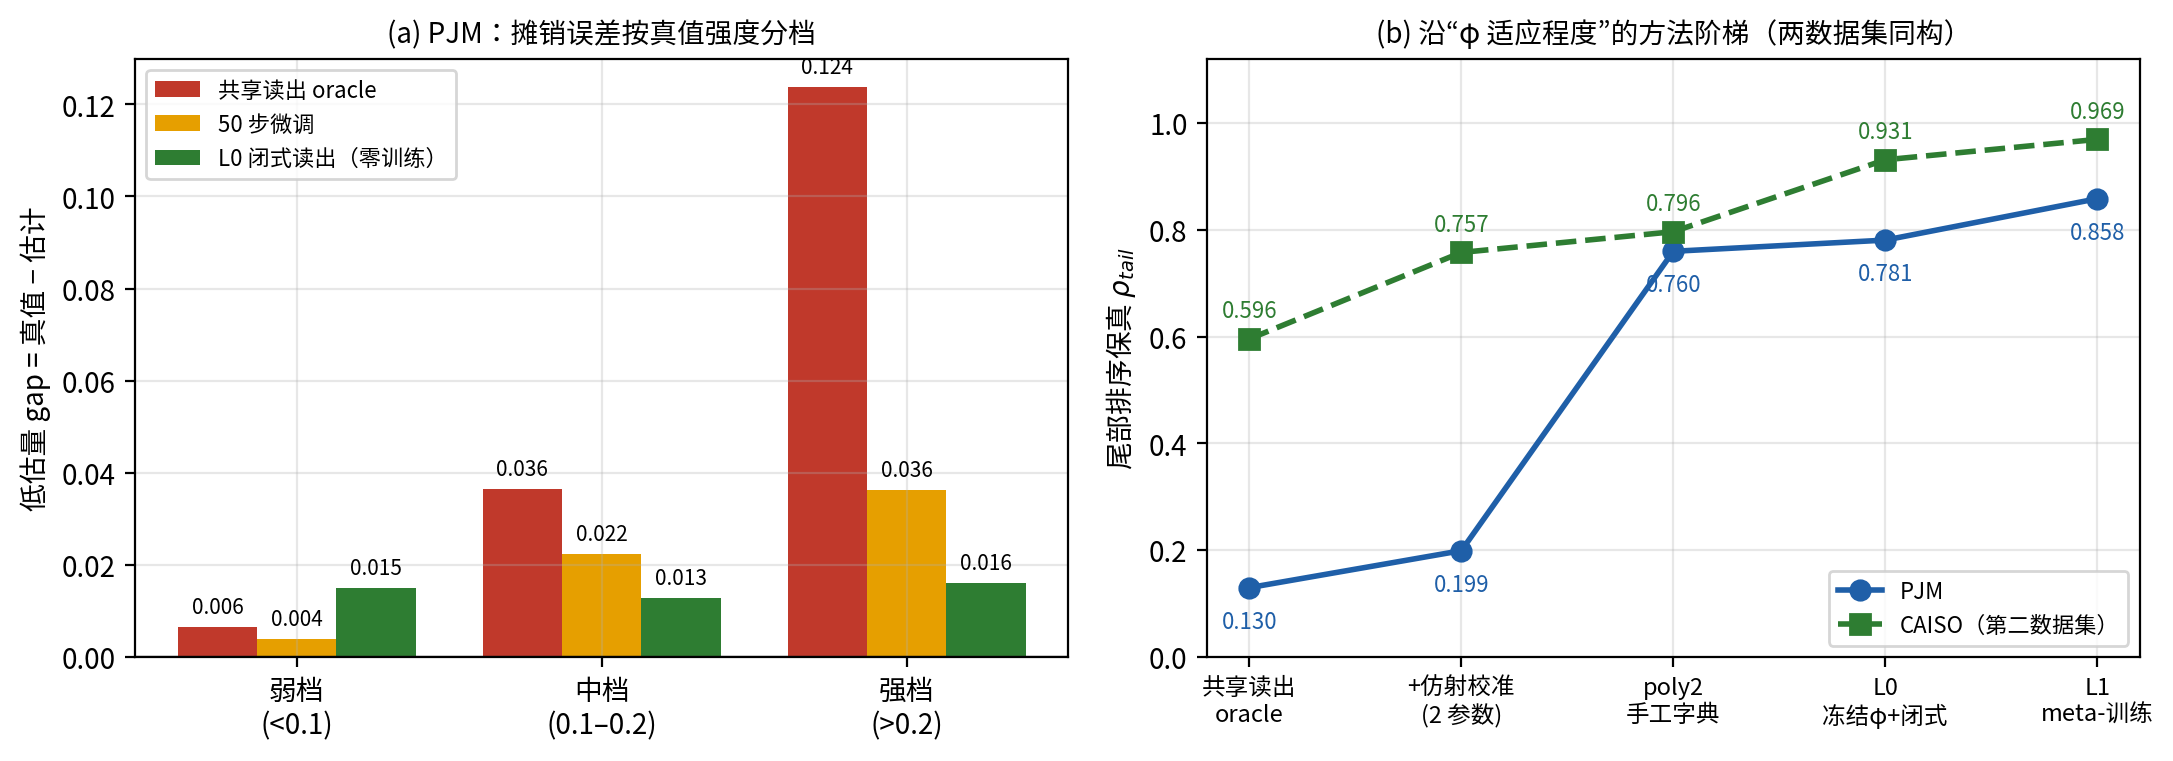
\includegraphics[width=0.99\linewidth]{gap_and_ladder.png}}
{\heiti 图 3\quad (a) PJM 单变量受控对照：低估量随真值强度分档（共享读出在强档低估 0.124，闭式读出降至 0.016，优于 50 步微调的 0.036）；(b) 两个数据集上的方法阶梯（尾部排序相关），形态同构}
\label{fig:ladder}
\end{figure*}

\subsection{RQ2：成本}

表 \ref{tab:cost} 与图 \ref{fig:cost} 给出三阶查询的实测成本。闭式读出 2.475 ms/集合，相对 25 步微调（55.5 ms）快 \textbf{22.4 倍}，同时精度更高；共享读出 oracle 虽然最快（0.32 ms），但如前所述在尾部不可用。这一“更快且更准”的组合正是把摊销放在表示层的直接收益：适应发生在闭式解里，而不是梯度步里。

\begin{table}[htbp]
\centering
{\heiti 表 2\quad 单集合查询成本与保真度（PJM，三阶，200 个集合实测）}
\label{tab:cost}
\vspace{2mm}
\zihao{5-}
\begin{tabular}{lccc}
\toprule
方法 & ms/集合 & 相对微调加速 & $\rho$ \\
\midrule
共享读出 oracle & 0.32 & 172.9$\times$ & 0.686 \\
25 步查询微调 & 55.49 & 1.0$\times$ & 0.876 \\
\textbf{L0 闭式读出} & \textbf{2.48} & \textbf{22.4$\times$} & \textbf{0.904} \\
\bottomrule
\end{tabular}
\end{table}

\begin{figure}[htbp]
\centering
\centerline{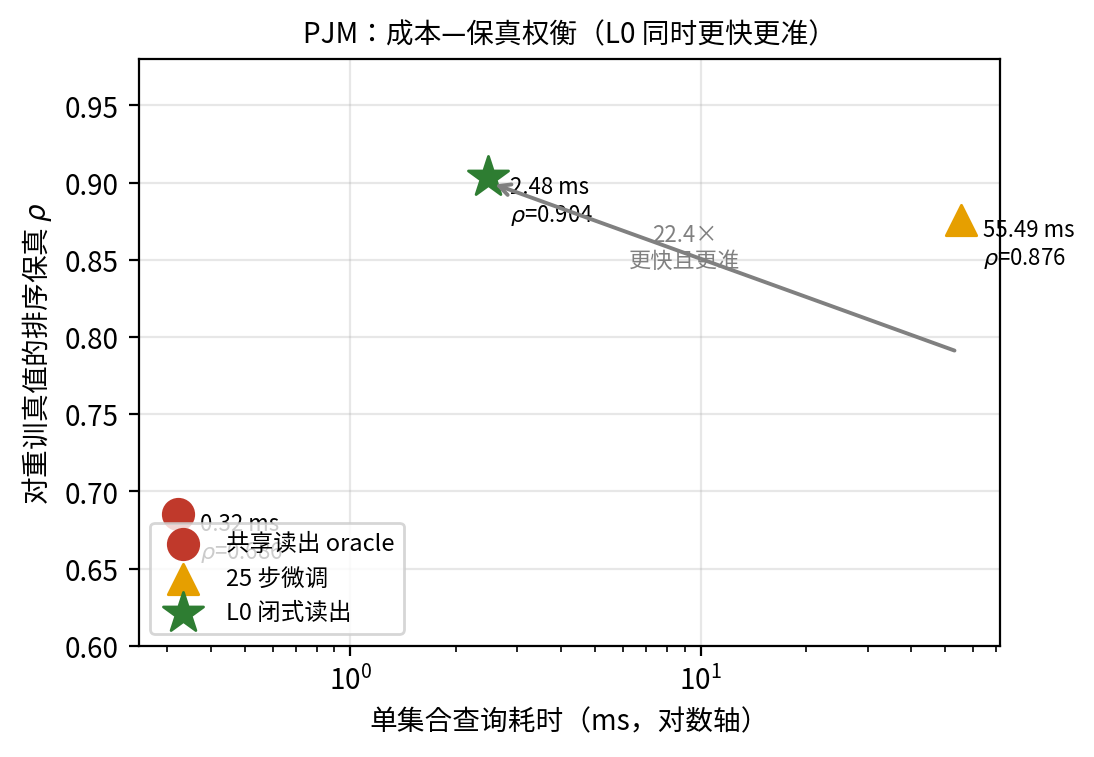
\includegraphics[width=0.82\linewidth]{cost_fidelity.png}}
{\heiti 图 4\quad 成本—保真权衡。闭式读出同时占据“更快”与“更准”}
\label{fig:cost}
\end{figure}

\subsection{RQ3：高阶决战——手工字典的认证级证伪}

高阶（四、五阶）没有现成真值，必须靠认证。本文让两个估计器各自\textbf{自选} top 候选，再送同一套重训认证流程，另配随机对照组（从弱估计集合中随机抽取），用 Mann--Whitney 单边检验判断强组是否真的强于对照。

结果构成本文最强的负面证据（图 \ref{fig:certify} 左、中）。手工 full 字典在五阶报出 441 个 $\syn>0.2$ 的强协同（最大 0.514），其 top-40 经重训认证后：认证均值仅 \textbf{0.031}，\textbf{无一超过 0.10}，65\% 的集合出现“子集反超”（某个四阶子集的真值反而高于五阶全集，即根本没有增量），与随机对照组\textbf{无统计差异}（$p=0.058$）。机制是清楚的：字典在小子集上过拟合，差分把过拟合量记成了“高阶增量”，且字典越复杂越严重。

同一空间上，L1 全枚举 108.6 万个五阶集合，报出的最大 $\syn$ 为 \textbf{零个超过 0.2}；其自选 top-21 经认证有 \textbf{10 个超过 0.10}（最强 0.154），显著强于 full 的 top（$p=0.013$）与随机对照（$p=0.003$），且真强的那一半估计几乎无偏（0.143 对 0.154）。四阶复现同一结论：full 的 top-20 认证后 0 个过 0.10，L1 的 top-20 有 9 个过 0.10（最强 0.196）。此外，L1 还\textbf{正确否决}了 full 的整个候选榜——full 的假 top-40 在 L1 的排序中位名次为 438504/1086008，前 1000 名内 0 个。

这里也须诚实报告 L1 的局限：图 \ref{fig:certify}(中) 显示其 top 候选呈\textbf{双峰}——一半认证为真（0.12--0.16），一半塌到 0.03 附近，单种子精确率约 48\%。这说明结构化估计仍只是\textbf{候选生成器}，而非终值；6.7 节给出把精确率提到 100\% 的过滤手段。

\begin{figure*}[htbp]
\centering
\centerline{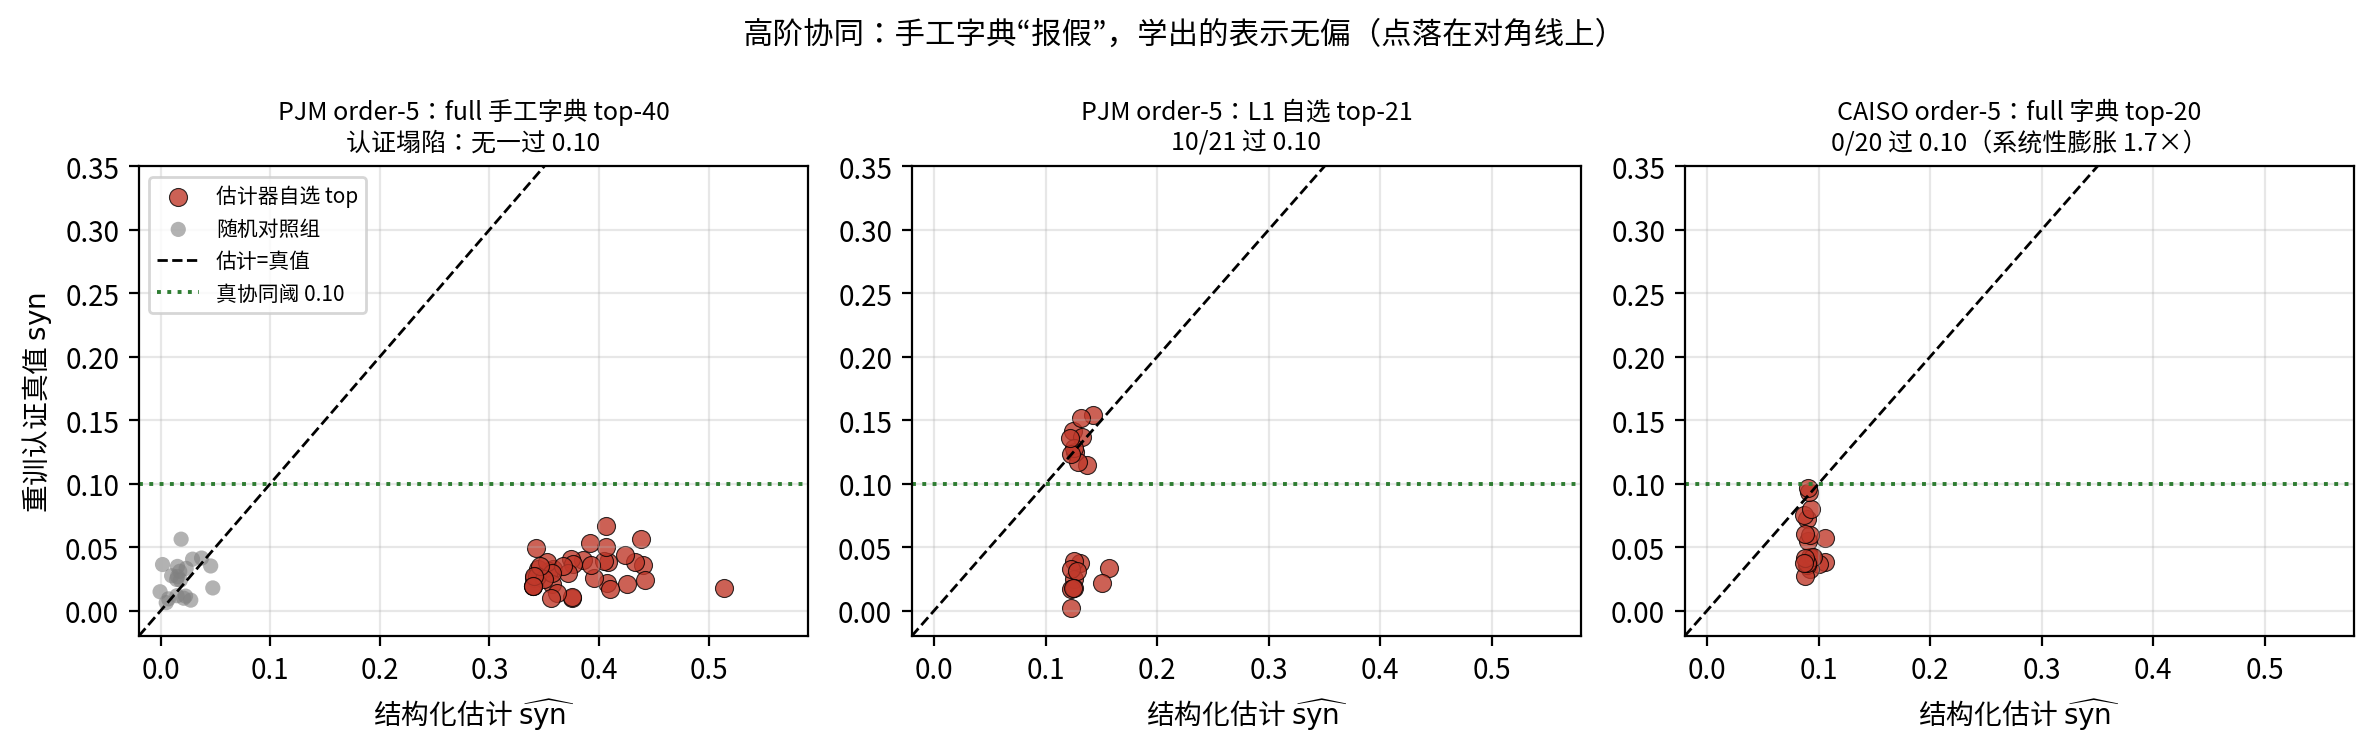
\includegraphics[width=0.99\linewidth]{certify_highorder.png}}
{\heiti 图 5\quad 五阶协同的重训认证。左：PJM 上手工字典 top-40 全部塌陷（点远离对角线且全在 0.10 以下）；中：L1 自选 top-21 有 10 个为真，呈双峰；右：CAISO 上字典同样 0/20 为真，并系统性膨胀 1.7 倍}
\label{fig:certify}
\end{figure*}

\subsection{RQ4：真值版衰减律与反层级协同}

以认证结果为准，本文给出协同强度与密度随阶数的定标（图 \ref{fig:decay}、表 \ref{tab:decay}）。PJM 上三至五阶的最强真值为 $0.455\to0.196\to0.154$（衰减 2.3 倍再 1.3 倍，温和单调），密度（$\syn>0.10$ 的比例）为 $0.498\%\to0.069\%\to0.0051\%$（每阶下降 7--13 倍）。三阶数字由两条独立路径互证：专用重训给 0.455，配对 FDR 的统计口径给 0.461。

\textbf{尺子本身随阶衰减（必须标注的口径）}。上述定标是用重训认证这把尺子量出来的，而第 \ref{sec:ceiling} 节的注入实验表明，这把尺子的\textbf{灵敏度本身随阶数下降}：注入已知强度的纯 $k$ 阶信号后，认证协议在五阶只量回 $0.30$--$0.39$ 倍、六阶 $0.25$--$0.28$ 倍。因此表 \ref{tab:decay} 中的衰减\textbf{混合了真实衰减与测量衰减}，其单调方向可信，但倍数是下界（真实的高阶强度可能高于表中数值，而不会低于）。这一口径先前未被披露，是本文在第二数据集与注入定标之后作出的修正。

该定标有直接的安全含义：\textbf{在可认证范围内（$k\le5$），最危险的协同是低阶的}。此限定不可省略——\ref{sec:notail} 节表明六阶及以上的协同虽然弱而普遍，其外推强度仍在显著阈之上，只是本文管线无法认证；把该结论读作"高阶安全"是错误的。同时它也修正了本文前置工作中两个先后出现的错误结论——基于 poly2 字典曾得到“三到四阶存在断崖式下跌”，基于 full 字典曾得到“高阶不衰减、风险被系统性低估”；认证表明两者都是\textbf{字典假象}。这段修正链本身是本文方法论主张的最好例证：没有重训认证做裁判，结构化估计的任何定量结论都可能是估计器的伪影。

\begin{table}[htbp]
\centering
{\heiti 表 3\quad 真值版衰减律（两个数据集，均以重训认证为准）}
\label{tab:decay}
\vspace{2mm}
\zihao{5-}
\begin{tabular}{lcccc}
\toprule
 & \multicolumn{2}{c}{PJM} & \multicolumn{2}{c}{CAISO} \\
\cmidrule(lr){2-3}\cmidrule(lr){4-5}
阶 $k$ & 最强真值 & 密度 & 最强真值 & 密度 \\
\midrule
3 & 0.455 & 0.498\% & 0.294 & 0.921\% \\
4 & 0.196 & 0.069\% & 0.157 & 0.031\% \\
5 & 0.154 & 0.0051\% & 0.104 & $\approx$0 \\
\bottomrule
\end{tabular}
\end{table}

\textbf{反层级协同}。ProxySPEX\upcite{kang2024proxyspex} 等高阶搜索依赖层级性假设：高阶强交互的低阶子集也应当强，从而可用 beam 搜索逐层展开。本文用\textbf{认证过的}真五阶协同直接测量该假设：10 个已认证真协同的最好四阶父集在四阶全扫中的排名为 164--2429，即 beam 宽度 $B=100$ 会全部漏掉、$B=1000$ 漏 4 个、$B=5000$ 才全覆盖。结论是双面的：反层级协同确实存在且幅度不可忽略，但由于 L1 查询仅 2.5 ms，$k\le5$ 可直接全枚举，因而该问题在本文管线中被\textbf{消解而非绕过}（$k\ge6$ 仍为开放问题）。

\begin{figure*}[htbp]
\centering
\centerline{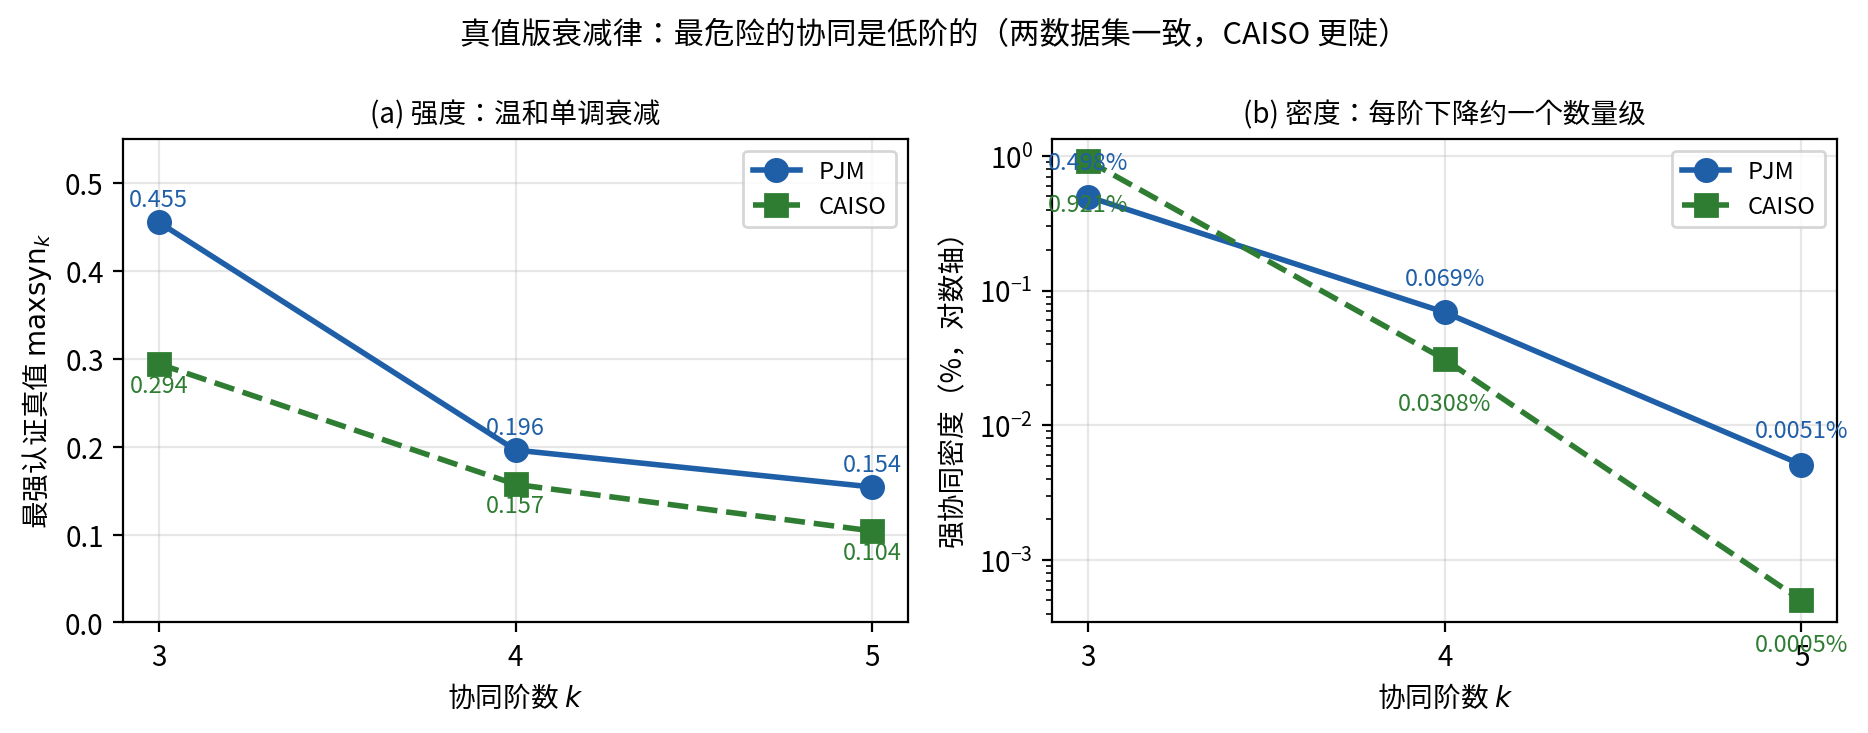
\includegraphics[width=0.92\linewidth]{decay_law.png}}
{\heiti 图 6\quad 真值版衰减律。(a) 最强协同强度温和单调衰减；(b) 强协同密度每阶下降约一个数量级。CAISO 比 PJM 更陡}
\label{fig:decay}
\end{figure*}

\subsection{RQ5：统计层——配对 FDR 的筛选力}

硬阈值“$\widehat{\syn}>\tau$”不带任何错误率保证。第 2 层的配对检验把它换成统计判断：PJM 三阶全扫的 13244 个三元组中，$\tau=0.10$ 的硬阈值给出 1924 个，过 BH-FDR（$q=0.05$）后只剩 \textbf{66 个（3.4\%）}；CAISO 上同一口径为 1526 个收缩到 122 个（图 \ref{fig:fdr}）。

一个值得记录的观察是：$\tau=0$ 的点零假设\textbf{没有筛选力}——PJM 上 57.5\%、CAISO 上 69.9\% 的三元组都能拒绝“增量为零”，因为“多给一个字段几乎总能带来一点统计可检测的信息”。审计要控制的错误是“声称 $\syn>\tau$ 但实际不足”，因此 $\tau$ 必须取审计真正关心的强度而非 0。

\begin{figure}[htbp]
\centering
\centerline{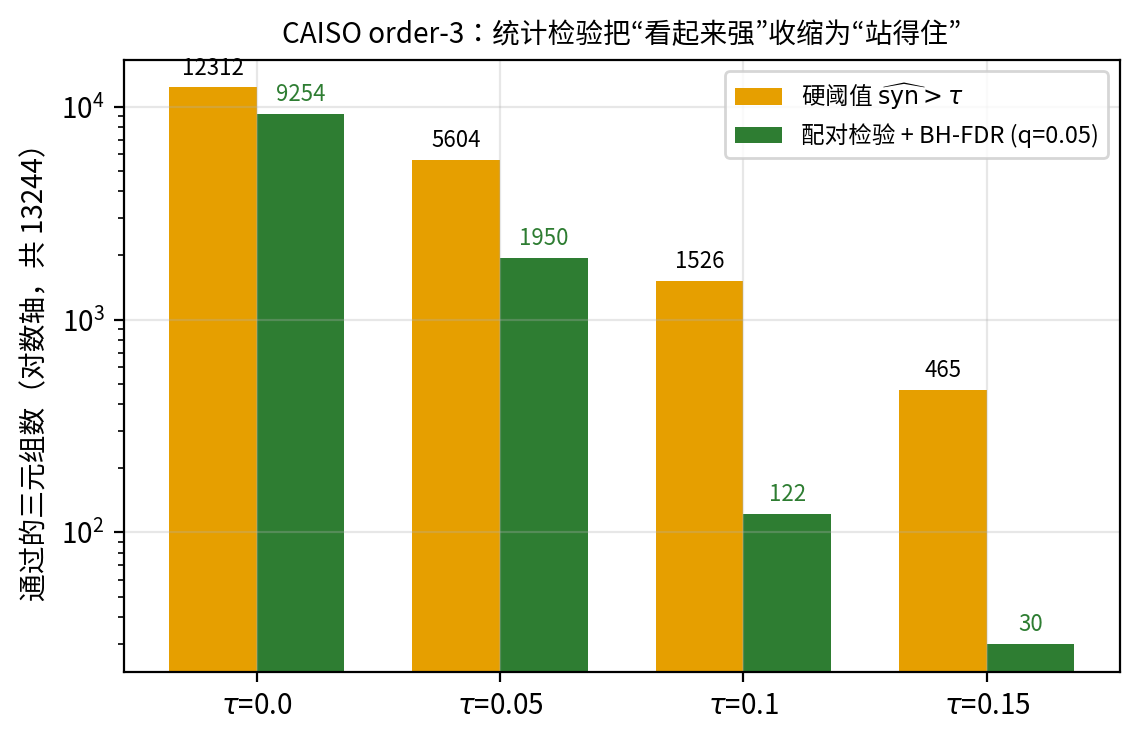
\includegraphics[width=0.8\linewidth]{fdr_filter.png}}
{\heiti 图 7\quad CAISO 三阶：配对检验 + BH-FDR 把“看起来强”收缩为“站得住”。$\tau=0$ 无筛选力}
\label{fig:fdr}
\end{figure}

\subsection{RQ6：跨种子秩一致性过滤}

RQ3 暴露的双峰问题需要一个 truth-free 的过滤器。本文的解法基于一个观察：真协同在\textbf{独立重训}的不同种子模型中都排在前面，而假候选的排名在种子间剧烈漂移。定义跨种子几何平均排名 $\mathrm{cr}(S)=\sqrt{r_1(S)\cdot r_2(S)}$，则 PJM 四阶认证批上真协同的 $\mathrm{cr}$ 中位数为 105、假候选为 27647，\textbf{分离 263 倍}；取阈值 $\mathrm{cr}\le500$ 后精确率由 45\% 提升至 \textbf{100\%}，召回 9/9 不损失（图 \ref{fig:ens}）。

这一结果与 4.2 节的对照 (2) 构成方法论上的呼应：\textbf{同族集成的方差}对摊销偏差失明（因为成员共享同一偏差），而\textbf{独立重训的秩一致性}恰好能打破它。对付共享偏差要用秩统计，不能用方差。诚实标注：该阈值是在同一批认证集合上选定的，需要前瞻验证；但 263 倍的分离幅度使结论对阈值极不敏感（300--1000 之间结果一致）。

\begin{figure*}[htbp]
\centering
\centerline{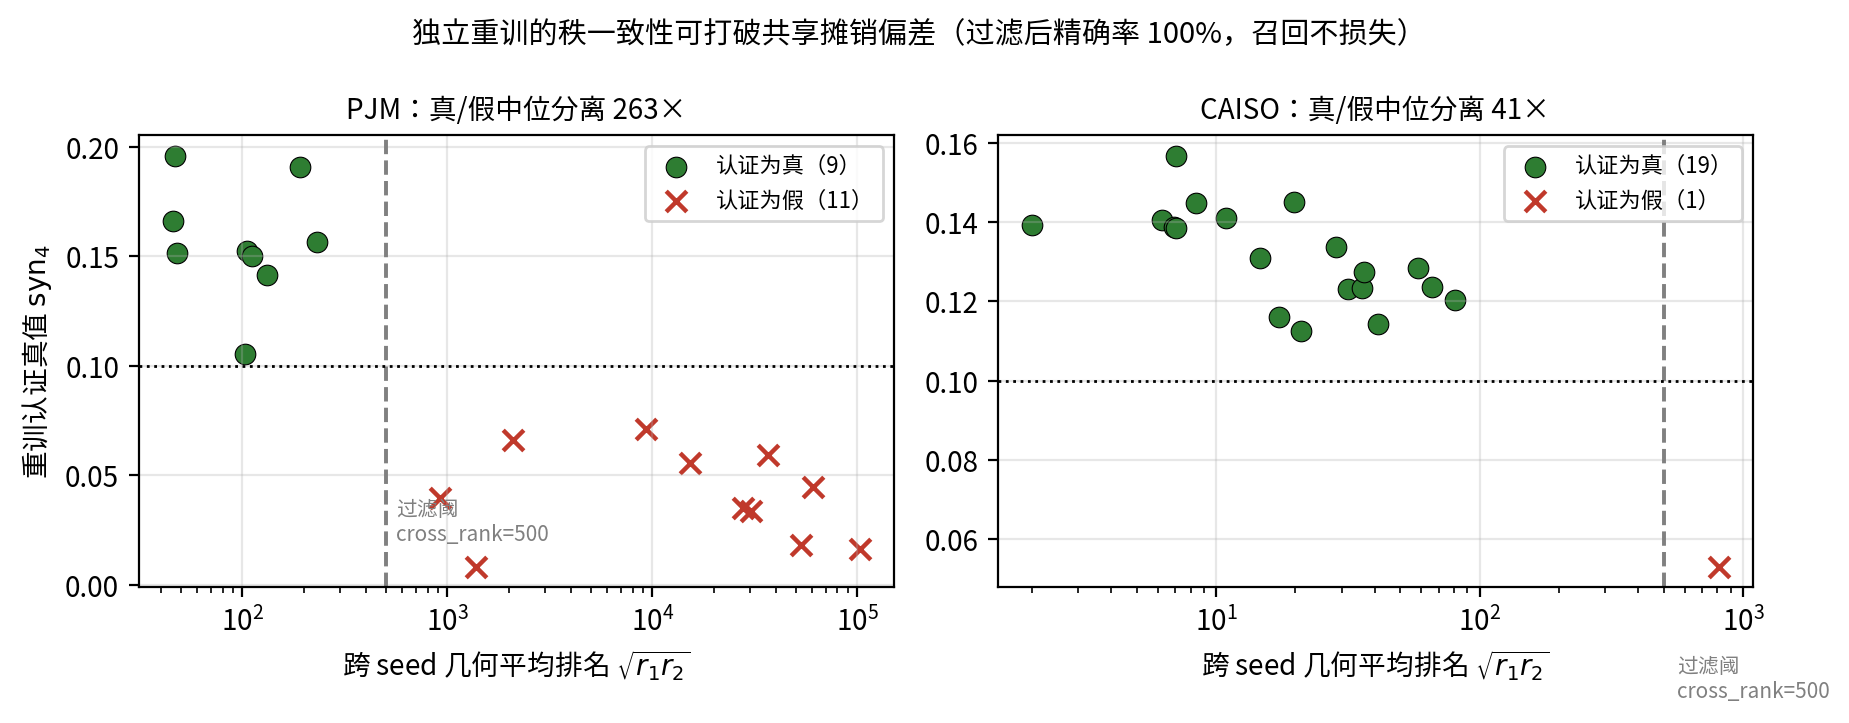
\includegraphics[width=0.92\linewidth]{ensemble_filter.png}}
{\heiti 图 8\quad 跨种子秩一致性过滤。真协同（圆点）集中在小 $\mathrm{cr}$ 区，假候选（叉号）漂移到大 $\mathrm{cr}$ 区}
\label{fig:ens}
\end{figure*}

\subsection{RQ7：第二数据集的完整复现}

为检验结论是否只是 PJM 的特性，本文在 CAISO 2025 数据上重跑整条管线，除字段设计外\textbf{零协议改动}。

\textbf{字段设计与泄露审计}。CAISO 原始表 307 列（35 个平衡区负荷、34 个日前负荷预测、分区风光实际与预测、三枢纽日前与实时 LMP 及其分量、日前计划的发用电与进出口、辅助服务需求与出清、实时区域间转移等）。为与 PJM 可比，收缩为 44 可见 + 12 机密，并做三轮泄露审计（判据：任一机密字段被 44 个可见字段线性重构的 $\Rtwo$ 不超过 PJM 轮廓的最大值 0.998）：第一轮发现实时电能分量可见时，机密的实时阻塞价格因 LMP 恒等式（总价 = 电能 + 阻塞 + 损耗 + 碳）几乎被精确重构（$\Rtwo=0.996$），故移出实时电能分量；第二轮发现三个内部分区实际负荷可见时，机密的系统总负荷被加和恒等式重构到 $\Rtwo=0.99998$，故换为三个外部平衡区负荷；第三轮发现两列辅助服务出清价全年恒为零（会被预处理当常量列删除，使字段数掉到 42），换为调频里程需求下限。最终最大线性泄露 0.989，轮廓跨度 0.24--0.99，与 PJM 的 0.28--0.998 形态一致。这一过程本身说明：\textbf{跨数据集迁移时，字段设计必须做恒等式级的泄露审计，否则“协同发现”可能只是在重新发现会计恒等式}。

\textbf{复现结果}。(1) 方法阶梯同构（图 \ref{fig:ladder}(b)）：共享读出 oracle 尾部 0.596，仿射校准 0.758，poly2 字典 0.796，L0 0.931，L1 0.969（三个种子 0.965--0.973）。三阶同构：oracle 0.424，字典 0.581--0.590，L0 0.766，L1 0.788。(2) 高阶认证（图 \ref{fig:caiso}）：L1 四阶自选 top-20 认证精确率 \textbf{19/20 = 95\%}，对照组 0/20，$p<0.0001$；五阶 top-21 的估计几乎无偏（结构化均值 0.076 对认证均值 0.075）。(3) 字典失效方向复现：full 字典五阶 top-20 认证 \textbf{0 个}为真，且系统性膨胀 1.7 倍（0.093 对 0.053）。(4) 衰减律复现且更陡（表 \ref{tab:decay}）。(5) 跨种子过滤复现：分离 41 倍，阈值 500 下精确率 100\%、召回不损失。

\textbf{两点实质差异}值得写入讨论。其一，CAISO 的衰减更陡：三阶密度是 PJM 的 1.85 倍，但五阶强协同几乎绝迹——协同谱的形状随数据集变化，而“低阶最危险 + 单调衰减”的定性结论稳定。其二，CAISO 上 L1 的单种子精确率高达 95\%（PJM 为 48\%），字典失效也更温和（无假阳性洪水，仅五阶膨胀）。这提示字典过拟合的幅度与数据的共线结构相关，应当削弱“手工字典必然大规模报假”这一强表述，改为“字典在高阶上的可靠性无保证，须逐数据集认证”。

\begin{figure*}[htbp]
\centering
\centerline{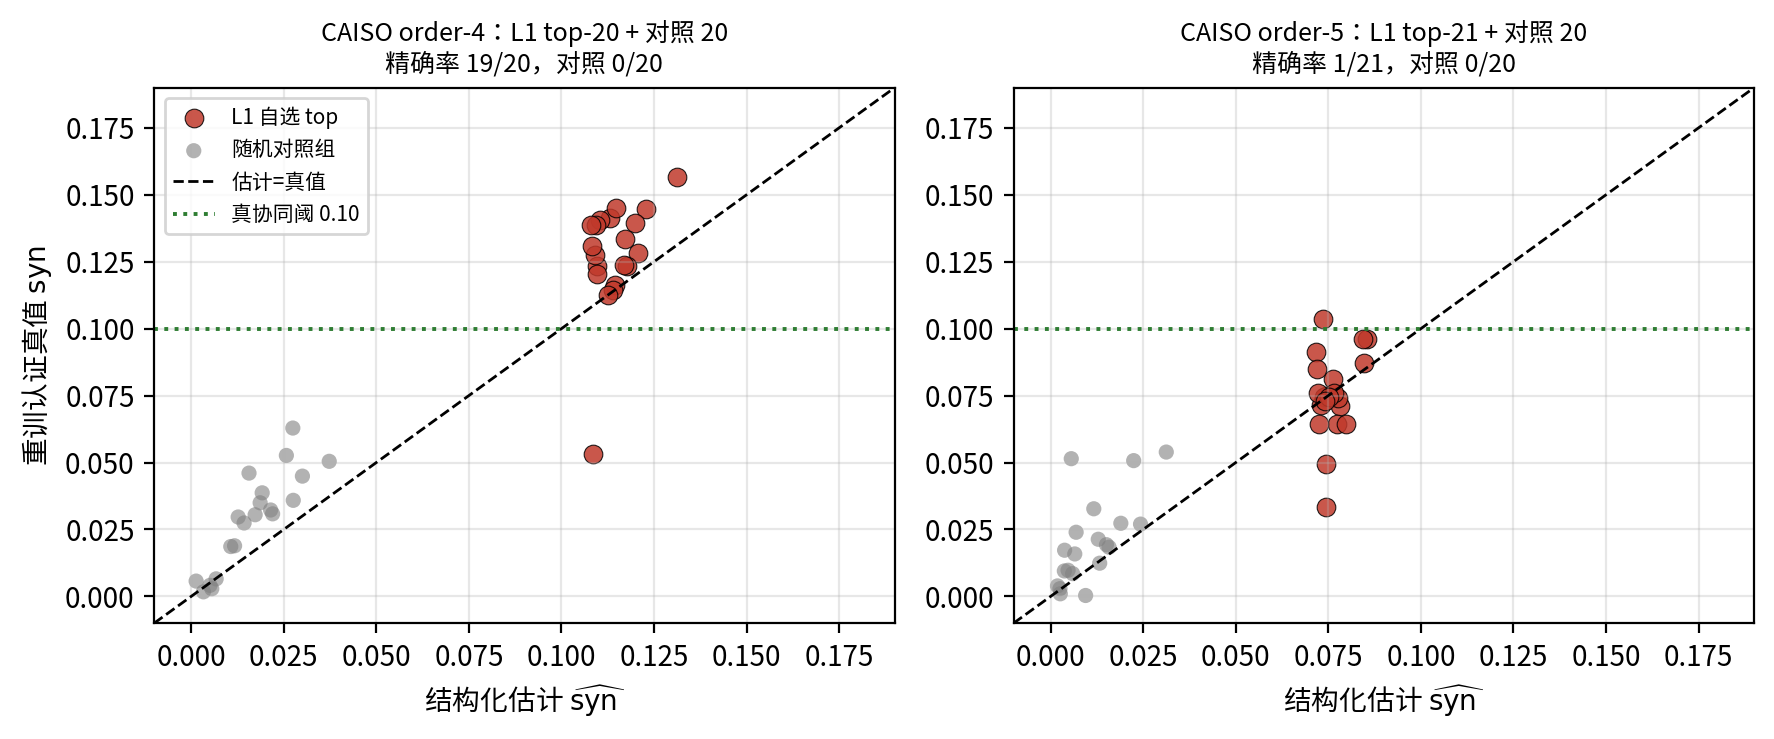
\includegraphics[width=0.86\linewidth]{caiso_certify.png}}
{\heiti 图 9\quad CAISO 上 L1 自选候选的重训认证。四阶精确率 19/20，五阶估计几乎无偏；两阶的随机对照组均为 0}
\label{fig:caiso}
\end{figure*}

\subsection{一个零成本基线：协同与共线性}

最后报告一个附带发现。在高斯线性假设下，可达 $\Rtwo$ 有闭式 $\Rtwo_c(S)=r^{\top}R^{-1}r$（$R$ 为可见字段相关阵、$r$ 为其与机密字段的相关向量），据此可零成本算出协同的线性代理。在 CAISO 二阶全空间上，该代理的尾部排序相关为 0.713，已\textbf{超过共享读出 oracle}（0.596）；在认证集合上判别“真协同”的 AUC 为三阶 1.000、四阶 0.962、五阶 0.825。这提示协同泄露在很大程度上是\textbf{共线性放大}的表现：当可见字段之间高度相关时，其相关阵求逆会放大与机密字段的联合投影。该基线不能取代学出的表示（尾部 0.713 对 0.97），但为“协同为何存在”提供了一个可解释的机制假说，也是一个便宜的预筛选器。

\subsection{RQ8：可认证边界 $k^\ast$ 与它的三段式成因}
\label{sec:ceiling}

前述结论均止于 $k\le5$。本节用\textbf{注入定标}回答一个更基本的问题：管线的可认证边界在哪里，以及卡住它的到底是什么。做法是向数据注入已知强度的纯 $k$ 阶信号
\begin{equation}
y \;=\; \alpha\cdot\mathrm{norm}\!\Big(\prod_{i\in S}\tanh(z_i)\Big) \;+\; \sqrt{1-\alpha^{2}}\,\varepsilon ,
\qquad \Rtwo_{\text{真}}=\alpha^{2},
\end{equation}
再分别问两端：\textbf{真值端}——重训认证能否把 $\alpha^2$ 量回来（量不回说明尺子的噪声底高于信号）；\textbf{搜索端}——摊销估计器给注入集合的 $\syn$ 在 400 个同阶随机集合中排第几百分位（低百分位说明搜索失明）。两端共用同一批元组，每阶 6 个，注入强度 $\alpha^2\in\{0.20,0.35\}$。

\textbf{注入构造的一处更正}。文献与本文前置实验常用的 $y=\alpha\cdot\mathrm{norm}(\prod_i z_i)$ 在真实电网字段上\textbf{并不是纯高阶交互}：原始乘积重尾极强（六阶峰度中位数 1127），被少数极端样本主导，而这些极端值由单个因子驱动，于是"交互项"退化为单字段的函数。自检可直接暴露该缺陷：二阶注入 $0.35$ 只量回 $0.028$。改用 $\tanh$ 压缩（有界单调）并加三重元组筛选（两两 $|\rho|<0.5$、乘积峰度 $<30$、单字段柔性解释力 $<0.05$）后，峰度降至 18，二阶自检量回 $0.29$--$0.34$。凡以旧构造得到的高阶注入结论均应按此更正重读。

\begin{table}[htbp]
\centering
{\heiti 表 4\quad 注入定标：可认证边界的两端（PJM / CAISO，注入 $\Rtwo=0.20$）}
\label{tab:ceiling}
\vspace{2mm}
\zihao{5-}
\begin{tabular}{lcccc}
\toprule
 & $k=5$ & $k=6$ & $k=7$ & $k=8$ \\
\midrule
真值端回收率 & 0.39 / 0.30 & 0.28 / 0.25 & 0.05 / 0.12 & 0.07 / $-$0.01 \\
单调性违反率 & 0\% / 0\% & 0\% / 0\% & 25\% / 33\% & 17\% / 50\% \\
搜索端 $\varphi$ 中位百分位 & 100 / 100 & 12 / 99 & 0.4 / 6.8 & 5.9 / 11.0 \\
搜索端 full 中位百分位 & 100 / 100 & 100 / 100 & \textbf{100 / 100} & 0 / 0 \\
\bottomrule
\end{tabular}
\end{table}

结果（表 \ref{tab:ceiling}）把 $k\ge6$ 的失败拆成三段，三段的成因互不相同：

\textbf{(a) $k\le5$：可认证。} 两端俱佳，与前文全部结论一致。

\textbf{(b) $k=6$--$7$：合成信号上卡在表征，真实字段上另有成因。} 真值端仍能量回（回收率 $0.25$--$0.28$，单调性违反率 $0\%$），说明尺子还没坏；而搜索端 $\varphi$ 在七阶跌到百分位 $0.4$--$6.8$（随机基线 50）。关键对照是：换成与目标无关的手工 full 字典，\textbf{同一批七阶信号仍被稳定挑到 400 个随机集合的第一名}（CAISO 六个元组 $6/6$ 命中，PJM $4/6$）。两臂唯一差别是特征基，因此六、七阶在\textbf{合成注入信号上}的搜索失败不能归因于阶数，而是 $\varphi$ 对未见过的交互型目标分布外。

这条诊断给出了一条可证伪的改进路线——把合成高阶信号混入 L1 的元训练任务分布——\textbf{本文把它执行到底，得到一个信息量更大的负结果}，详见 \ref{sec:transfer} 节。

\textbf{(c) $k\ge8$：统计硬墙。} 连含有生成单项式的 full 字典也塌（中位百分位 0），真值端回收率归零、单调性违反率升至 $17\%$--$50\%$。三项排除性证据表明这是样本量决定的可学性极限而非实现问题：换更大攻击者（$512\times3$ MLP）或梯度提升树均无改善（学到比例 $0.64/0.62/0.23$）；样本量缩放显示六阶的学到比例在 $n=3600$ 仍在陡升尚未饱和；$6105$ 行的 CAISO 在每一阶都略优于 $4589$ 行的 PJM。

\textbf{结论}：本文管线的可认证边界为 $\boldsymbol{k^\ast=5}$，两数据集一致；但该边界在六、七阶由\textbf{表示}决定（可改进），到八阶才由\textbf{样本量}决定（短期无解）。

\textbf{此对照不可外推的方向}。full 字典显式含有生成信号所用的那个 $k$ 阶单项式，对本合成信号近乎\textbf{配基}，故表 \ref{tab:ceiling} 比较的是"基是否匹配"，而非"哪个字典在真实数据上更好"——后者已在 RQ3 中被认证否决（真实机密字段上 full 的五阶 top 与随机对照无差异）。可稳健外推的只有 (c) 段的硬墙结论（连配基都失败）与 (b) 段的\textbf{否定形式}（六、七阶的失败不能归因于阶数）。

\subsection{改进路线的执行与零迁移：注入定标高估真实能力}
\label{sec:transfer}

上节把 $k=6$--$7$ 的失败归因于 $\varphi$ 的表征，并指向"改造元训练任务分布"。本文执行了这条路线，其结果同时修正了一条既有局限、又暴露出一个方法学陷阱。

\textbf{起点是一个实现缺陷。} 前置工作曾试过用合成目标增广元训练，结论是"修不好、属容量竞争"（本文早期版本的局限 (1)）。复查发现该实现对 support 集与 query 集\textbf{各自独立抽取}字段元组，致使同一合成列在两端对应不同元组——闭式读出在 support 上拟合元组 $A$、却在 query 上对元组 $B$ 计损失，该损失项\textbf{不可约}。修正后做四臂消融（每格 $3$ 种子 $\times$ $24$ 元组 $=72$ 次注入，命中定义为百分位 $\ge95$）：不增广臂与带缺陷增广臂在各阶均无显著差异（$p\ge0.30$），\textbf{证实"带缺陷的增广等于没做"}；仅修此一处，$k=6$ 命中率由 $32\%$ 升至 $75\%$、$k=7$ 由 $10\%$ 升至 $28\%$（Fisher 单侧 $p<0.01$），且二阶真实机密字段的尾部相关不退化（各臂 $0.79$--$0.85$，落在种子噪声带内）。值得注意的是，该臂训练时只见过二至四阶合成目标而测试在五至七阶，属\textbf{跨阶泛化}。

\textbf{但增益不迁移到真实机密字段。} 用修好的 $\varphi$ 在真实六阶空间重扫并认证，与原 $\varphi$ 共用同一候选池（$30$ 万个六阶集合，同随机种子），唯一变量是特征基。扫描端新 $\varphi$ 确实报出更强候选（池内最大估计 $0.148$ 对 $0.107$，超阈候选 $3\to9$）；\textbf{认证端却归零}：top-10 认证均值由 $0.031$ 降至 $0.016$，与对照组无法分开（AUC $0.30$，Mann--Whitney $p=0.98$），新旧 top 的认证差异不显著（$p=0.24$）。

\textbf{这构成一个直接的方法学警示}：用合成注入信号定标高阶发现能力是本领域的通行做法，而此处合成端 $32\%\to75\%$ 的显著提升在真实端\textbf{完全不存在}。注入信号是乘积型、强度 $0.20$--$0.35$，与手工字典和改造后的 $\varphi$ 都近乎同构；真实高阶协同既非此形状、强度也低得多。因此\textbf{注入定标给出的是能力上界，不应被读作真实场景的性能预期}——表 \ref{tab:ceiling} 的全部数字都须在此意义下理解。

\subsection{排除认证协议：噪声底不是选择偏差}

零迁移还剩一个竞争解释：也许真实六阶协同存在，只是认证协议的噪声底（随机对照组认证均值约 $0.031$）把它淹没了。该噪声底有一个自然嫌疑——$\mathrm{syn}$ 的定义含两次取最大（对 $12$ 个机密字段、对 $k$ 个子集），在有限审计样本上会产生系统性正偏。

本文据此构造\textbf{配对认证协议}：机密字段 $c^\ast$ 与对比子集 $T^\ast$ 都在测试集的\textbf{搜索半份}上选定，只在\textbf{审计半份}上报增量，并对 $R=3$ 个重训种子取均值。协议先过硬闸门：在已有 $10$ 个认证为真的五阶协同上，配对口径\textbf{一个不丢}（$10/21$，与原口径的排序相关 $\rho=0.926$），证明协议在有信号处可靠。

但在六阶上，\textbf{噪声底纹丝不动}：对照组均值 $0.0314\to0.0338$（不降反升），top 与对照仍无法分开（AUC $0.23$）。这直接证伪了"噪声底 = 选择偏差"。同时，种子间标准差仅 $0.004$--$0.009$，比 $0.031$ 小 $4$--$7$ 倍，说明它也不是重训随机性。第三个候选解释——$v$ 在六阶已饱和至 $0.944$ 故增量被压缩——同样被证伪：$\rho(v_{\mathrm{true}},\mathrm{syn}_{\mathrm{true}})=+0.34$（六阶）与 $+0.50$（五阶），皆为正。

\subsection{真正的原因：高阶协同弱而普遍，没有强尾}
\label{sec:notail}

排除了重训方差、选择偏差与饱和压缩之后，剩下的解释是那个 $0.03$ \textbf{本来就是真的}。检验随机对照组的认证增量是否显著大于零：

\begin{center}
\begin{tabular}{lcc}
\toprule
& 均值 & 单样本 $t$ 检验（$>0$）\\
\midrule
六阶随机对照（原口径） & 0.0314 & $t=6.86$, $p<10^{-4}$\\
六阶随机对照（配对口径） & 0.0338 & $t=4.39$, $p=0.0009$\\
七阶随机对照（原口径） & 0.0224 & $t=6.72$, $p<10^{-4}$\\
\bottomrule
\end{tabular}
\end{center}

\textbf{随机抽取的六阶、七阶集合，其认证增量都显著大于零。} 按该阶的注入回收率反推，认证值 $0.03$ 对应真实强度约 $0.11$。也就是说，高阶协同并非稀少，而是\textbf{普遍存在且强度均匀偏弱}——分布向一个狭窄的弱值带收缩，\textbf{没有可供搜索的强尾}。top 与随机对照分不开，不是因为搜索失败，而是因为\textbf{两者本就没有实质差别}。

这给衰减律一个更强的形式：衰减的不只是最强值，而是整个分布的形状。它也解释了为何三条改进路线（更好的表征、更低的噪声底、更大的搜索预算）在六阶上全部无效——它们都在解决"找不到"的问题，而真实的问题是"没有值得找的"。

\subsection{估计器高估的性质：它是保守的，且随阶失去信息}
\label{sec:bias}

结构化估计在高阶上系统性高估认证真值，这本身需要交代清楚，否则前述结论会被质疑“用一把已知不准的尺子下结论”。

\begin{center}
\begin{tabular}{lccccc}
\toprule
阶 & 估计均值 & 认证均值 & 膨胀比 & 绝对高估 & $\max(\text{认证}-\text{估计})$\\
\midrule
$k=3$ & 0.306 & 0.279 & 1.10 & 0.027 & ---\\
$k=4$ & 0.147 & 0.093 & 1.58 & 0.054 & $+0.053$（$7/20$ 超出）\\
$k=5$ & 0.130 & 0.077 & 1.70 & 0.054 & $+0.020$（$7/21$ 超出）\\
$k=6$ & 0.102 & 0.031 & 3.28 & 0.071 & $\boldsymbol{-0.012}$（$0/10$）\\
$k=7$ & 0.066 & 0.013 & 5.25 & 0.054 & $\boldsymbol{-0.041}$（$0/10$）\\
\bottomrule
\end{tabular}
\end{center}

三点值得强调。第一，\textbf{膨胀比的爆炸是分母造成的}：绝对高估在 $k=3$--$7$ 上近似恒定（$0.027$--$0.071$），真值在缩小，比值自然显得越来越大。第二，\textbf{在 $k\ge6$ 上估计值是认证真值的经验上界}：连同 \ref{sec:fullspace} 节的 E3，$k=6$--$7$ 累计 $32$ 个集合\textbf{无一例外}，认证值都低于其估计值。也就是说估计器在高阶\textbf{只虚报、不漏报}——对安全审计而言这是正确的偏向。第三，\textbf{偏差的来源可定位}：估计器对全集的 $v$ 跟踪良好（差 $-0.003$ 至 $-0.012$），却大幅低估\textbf{最强子集}的 $v$（差 $-0.07$ 至 $-0.15$）；$\mathrm{syn}$ 是差分，减数偏小则差值虚高。这解释了偏移量为何与阶数基本无关——它来自子集拟合的系统性不足，而非阶数本身。（两项不精确相加，因为逐机密字段的 $\arg\max$ 不对齐；方向是可靠的。）

但 \ref{sec:fullspace} 节将表明，这一“常数偏移”的刻画在\textbf{极尾处失效}，届时给出更准确的描述。

\subsection{把“没有强尾”证到全空间：三个互不依赖的实验}
\label{sec:fullspace}

上节的结论依赖两个可质疑之处：所用随机对照抽自估计器判定的 $\mathrm{syn}<0.05$ 区间（\textbf{被估计器条件化过}），且全部结论建立在 $30$ 万个六阶集合的抽样池上（占全空间 $4.25\%$）。本文用三个实验把这两处补严。

\textbf{E1：六阶全枚举。} 对全部 $C(44,6)=7{,}059{,}052$ 个集合求结构化估计。全空间估计最大值为 $0.2299$，而 $4.25\%$ 抽样池只给出 $0.1475$——\textbf{抽样对极值统计量是不可靠的}（均值与分位数则稳定）。全空间中估计超过 $0.10$ 的仅 $312$ 个（$0.0044\%$），超过 $0.20$ 的仅 $2$ 个，密度极稀。

\textbf{E2：均匀随机集合的认证。} 独立于估计器均匀抽取 $18$ 个六阶集合并重训认证（$R=3$ 种子）。认证均值 $0.0204$、中位 $0.0205$、最大 $0.0428$、标准差 $0.0101$，\textbf{无一超过 $0.10$}；单样本 $t$ 检验 $t=8.56$、$p<10^{-5}$，显著大于零。与估计器挑出的 top-10（认证均值 $0.0310$）相比，\textbf{Mann--Whitney $p=0.433$，无差异}。

\textbf{E3：全空间极尾的认证。} E1 找出的 $312$ 个高分候选此前从未被认证（已认证的最强估计仅 $0.1195$，来自抽样池）。取全枚举 top-12（估计 $0.156$--$0.230$）送重训认证：认证均值 $0.0208$、最强 $0.0439$、\textbf{无一超过 $0.10$}，$\rho(\text{估计},\text{认证})=-0.056$，与 E2 的均匀随机集合相比 $p=0.576$，仍无差异。\textbf{全空间 $706$ 万个集合中估计最高的那一个（$0.2299$），认证值是 $0.0080$——低于随机抽样的中位数。}

三条腿对估计器的依赖程度递减：E1 完全依赖，E3 仅用它选候选，\textbf{E2 完全不依赖}。三者一致指向同一结论：六阶协同\textbf{普遍存在（$p<10^{-5}$）、强度均匀（$0.02\pm0.01$，按回收率反推真实强度约 $0.07$）、没有可检出的尾巴}。

\textbf{此处必须给出诚实的统计边界}：$18$ 个均匀随机样本全部不超过 $0.043$，据此对 $P(\mathrm{syn}>0.043)$ 的 $95\%$ 上置信界为 $15.3\%$——样本量只支持到这个精度，\textbf{不能宣称“绝对不存在强六阶协同”}。可以断言的是：在估计器能排进全空间前 $12$ 名的候选中不存在，且无条件分布集中于 $0.02$。

\textbf{一处必要的更正}。E1 之前，本文曾用一个“面值论证”支持结论——“六阶估计最大值 $0.1475$ 已低于五阶\textbf{认证}最大值 $0.1543$，故即使完全不修正高估，结论也不变”。全枚举表明该论证\textbf{建立在抽样假象上}（真实的全空间估计最大值为 $0.2299$），故予以撤回。同样地，\ref{sec:bias} 节的常数偏移模型在极尾处失效：E3 这批候选的绝对高估达 $0.154$ 而非 $0.055$。正确的刻画是：六阶的估计值\textbf{不是“真值加一个常数偏移”，而是“真值（近似常数）加纯噪声”}，估计越极端，其中噪声成分越大——$\rho=-0.056$ 正是此意。

\textbf{$\boldsymbol{k^\ast=5}$ 的三条独立依据}由此完整：(i) 搜索端不是瓶颈（配基字典在七阶仍 $100\%$ 命中）；(ii) 真值端在 $k\ge7$ 失效且受样本量限制（回收率 $\le0.12$、单调性违反 $25\%$--$100\%$）；(iii) \textbf{分布端在 $k\ge6$ 没有强尾}（本节，全空间已验）。前两条说"测不到"，第三条说"没有值得测的"。

\textbf{一处必要的措辞区分}。以上不等于"高阶没有协同"。灵敏度分析（可检测下限 $=2\times$ 噪声底 $\div$ 回收率）给出：PJM 在五阶余量 $2.2\times$、六阶 $1.4\times$、七阶仅 $0.25\times$；CAISO 六阶已降至 $0.9\times$。而按衰减律外推，七阶真实最强协同约 $0.25$（PJM）与 $0.15$（CAISO），\textbf{均在本文所用的 $0.10$ 显著阈之上}。因此正确的表述是\textbf{"存在但不可认证"}，而非"不存在"——在安全语境下这两句话含义相反。

%%%%%%%%%%%%%%%%%%%%%%%%%%%%%%%%%%%%%%%%%%
\section{\heiti 讨论}

\subsection{方法学教训}

本文的结论链条中有三处“先错后纠”，其修正过程各产出一件可复用的方法学工具，值得单独记录。

\textbf{(1) 置换检验对差分统计量有结构盲点}。为验证高阶发现的显著性，一个自然做法是打乱机密字段后重扫，看还能否找到同等强度的协同。本文曾以此认定 full 字典的高阶发现为真（置换后假发现率为 0）。但重训认证表明这些发现全假。原因是：打乱后 $v(S)$ 与 $v(T)$ \textbf{一起}归零，差分自然消失；而真实数据上两者都有信号时，差分的系统性偏差不会被置换检验暴露。教训是：\textbf{对差分统计量，置换检验可以给出误导性的通过}。

\textbf{(2) 注入实验区分“数据里没有”与“方法找不到”，但它只给上界}。当搜索不到强高阶协同时，需要判断是数据本身稀疏还是估计器失明。做法是人工注入已知强度的合成协同信号，看方法能否找回。本文正是用它推翻了先前“高阶不可能被搜到”的不可能性论证。

然而 \ref{sec:transfer} 节给出了这件工具的\textbf{使用边界}：改造表征使六阶注入命中率由 $32\%$ 翻倍至 $75\%$（$p<0.001$，每格 $72$ 次注入），而同一改造在真实机密字段上带来的认证增益\textbf{为零}。原因是注入信号必然要写成某种显式形式（此处为乘积型、强度 $0.20$--$0.35$），从而与手工字典或经同类信号训练的表征\textbf{近乎同构}，而真实协同既非该形状、强度也低一个量级。故注入实验能可靠地回答\textbf{否定性}问题（“连注进去的都找不回，则方法确有盲区”），却不能把肯定性结果外推为真实性能——\textbf{注入定标给出的是能力上界}。这一点对以合成基准评估高阶交互发现的通行做法是一个直接的警示。

\textbf{(2') 排除性实验优于解释性叙述}。本文对六阶噪声底提出过三个解释——选择偏差、重训方差、饱和压缩——并各设计了一个能证伪它的测量（配对协议、多种子标准差、$\rho(v,\mathrm{syn})$ 的符号）。三个全被推翻，剩下的解释“它本来就是真的”才因此可信（\ref{sec:notail} 节）。若只做支持性检验，任一解释都能被讲得头头是道。

\textbf{(3) 重训认证是唯一裁判}。结构化估计的一切定量结论——强度、密度、排序、显著性——在没有认证前都只是候选。本文的衰减律经历了“断崖 $\to$ 不衰减 $\to$ 温和衰减”两次反转，每次反转都由更强的证据推翻更弱的证据。

\subsection{局限}
\label{sec:limit}

(1) \textbf{$\varphi$ 不是通用基}。对分布外的合成目标信号，L0/L1 明显不如手工 full 字典（92 对 56 百分位）。\ref{sec:transfer} 节表明这条局限\textbf{在合成信号上可被修复}（修正元训练实现后 $k=6$ 命中率 $32\%\to75\%$），但修复\textbf{不迁移到真实机密字段}。因此本条局限的准确表述是：$\varphi$ 对合成交互目标的分布外问题源于训练任务分布、可以改造；而真实高阶场景的瓶颈不在此处（见局限 (4)）。两类基互补而非替代，实践中可考虑显式混合。

(2) \textbf{单种子候选精确率仍不足}（PJM 48\%），结构化估计只是候选生成器；跨种子过滤在认证样本上修到 100\%，但阈值需要前瞻验证。

(3) \textbf{高阶密度是估计而非全认证}：四、五阶密度由“估计器超阈计数 $\times$ 认证精确率”外推得到，三阶则有 FDR 的统计保证。

(4) \textbf{$k\ge6$ 未解决，成因有三层}：全枚举在六阶起不可行，而反层级协同的存在使 beam 搜索不可靠；第 \ref{sec:ceiling} 节表明合成信号上六、七阶的瓶颈在 $\varphi$ 的表征，八阶起是样本量决定的统计极限。但 \ref{sec:transfer}--\ref{sec:notail} 节表明，在\textbf{真实}机密字段上前两层都不是主因：改造 $\varphi$ 使合成端命中率翻倍而真实端毫无变化，降低认证协议噪声底亦然；真正的原因是六阶及以上的协同\textbf{弱而普遍、没有强尾可供搜索}。因此 $k\ge6$ 上"提升方法"这一方向本身收益有限，可行的只有扩大数据规模。

(4') \textbf{衰减律的尺子随阶衰减}：表 \ref{tab:decay} 的数字由重训认证量得，而该协议在五、六阶只回收注入强度的 $0.25$--$0.39$ 倍，故所报衰减混合了真实衰减与测量衰减，倍数应读作下界。

(5) \textbf{数据口径}：CAISO 的总发电量与联络线功率只有日前计划口径（无实时实测），系统损耗无对应字段，其“运行敏感性”语义弱于 PJM 一档。

(6) 本文的攻击者模型限于监督回归族，未考虑利用时序结构或外部辅助数据的更强攻击者。

%%%%%%%%%%%%%%%%%%%%%%%%%%%%%%%%%%%%%%%%%%
\section{\heiti 结论}

本文研究了数据推断泄露审计中集合敏感度 $v_c(S)$ 的忠实估计问题。核心发现是：把“集合 $\mapsto$ 敏感度”整体摊销进共享模型时，其误差系统性地集中在最危险的强协同集合上（尾部排序相关由全局的 0.606 坍缩至 0.130），且这一失效源于摊销层次的错配而非训练不足——$v_c(S)$ 是内层优化的最优值，摊销间隙在“最优解离共享平均解最远”的实例上最大，而协同的差分结构进一步放大了它。据此本文把摊销层次由“值”上移到“表示”，让读出权重按集合闭式重解，在零额外训练下即把尾部排序相关提升至 0.781、最强档低估由 0.124 降至 0.016，性能超过 50 步微调而快 22.4 倍。

在此基础上构建的“摊销扫描—配对 FDR—重训认证”三层管线，使 $k\le5$ 的协同发现无需依赖层级性假设，并给出了三项经认证的定量结论：手工多项式字典在高阶上既报假（五阶 441 个强协同认证后无一为真）又漏真；真值版衰减律为 $0.455\to0.196\to0.154$，密度每阶降约一个数量级，即最危险的协同是低阶的；跨独立种子的秩一致性可把候选精确率由 45\% 提升至 100\%。全部结论在第二个电网数据集上完整复现，且两处实质差异（衰减更陡、字典失效更温和）提示协同谱的形状与数据的共线结构相关。

最后，本文用注入定标给出了管线的可认证边界 $k^\ast=5$，并把边界之外的失败归因层层剥开。合成信号上，六、七阶的瓶颈在摊销表示对未见交互目标的分布外，八阶起则是样本量决定的统计极限。本文把由此指向的改进路线执行到底：修正元训练实现中的一处缺陷后，六阶注入命中率由 $32\%$ 升至 $75\%$——\textbf{但该增益在真实机密字段上完全不迁移}（认证均值 $0.031\to0.016$，AUC $0.30$）。进一步构造配对认证协议排除了"噪声底源于选择偏差"，饱和压缩亦被证伪。剩下的解释经检验成立：\textbf{随机抽取的六阶、七阶集合本身就带有显著大于零的协同增量}（$0.031$ 与 $0.022$，$p<10^{-4}$），即高阶协同弱而普遍、\textbf{没有强尾可供搜索}——六阶上的诸多改进之所以无效，是因为问题不在"找不到"，而在"没有值得找的"。

这条结论同时带来两处必要的措辞纪律。其一，"最危险的协同是低阶的"必须限定为"在可认证范围内"：外推显示七阶最强协同仍在显著阈之上，正确的表述是\textbf{"存在但不可认证"}而非"不存在"。其二，注入定标给出的是能力上界而非真实性能预期——合成端翻倍的增益在真实端为零，这对以合成基准评估高阶交互发现的通行做法是一个直接的警示。连同"认证尺子随阶衰减、所报衰减律倍数应读作下界"这一口径更正，三者共同说明：在这一问题上，任何定量结论都必须连同量它的那把尺子、以及那把尺子所处的分布一起报告。

未来工作包括：六阶及以上的可扩展发现、通用基与任务基的显式混合、跨种子过滤阈值的前瞻验证，以及把认证清单转化为最小防护集的组合优化。

\vskip 5mm
\noindent{\heiti 参考文献}
\vspace{2mm}
\zihao{5-}
\bibliographystyle{gbt7714-numerical}
\bibliography{ref}

\end{document}
